%%%%%%%%%%%%%%%%%%%%%%%%%%%%%%%%%%%%%%%%%
% University/School Laboratory Report
% LaTeX Template
% Version 3.1 (25/3/14)
%
% This template has been downloaded from:
% http://www.LaTeXTemplates.com
%
% Original author:
% Linux and Unix Users Group at Virginia Tech Wiki 
% (https://vtluug.org/wiki/Example_LaTeX_chem_lab_report)
%
% License:
% CC BY-NC-SA 3.0 (http://creativecommons.org/licenses/by-nc-sa/3.0/)
%
%%%%%%%%%%%%%%%%%%%%%%%%%%%%%%%%%%%%%%%%%

%----------------------------------------------------------------------------------------
%	PACKAGES AND DOCUMENT CONFIGURATIONS
%----------------------------------------------------------------------------------------

\documentclass{article}
\usepackage[left=4cm, right=4cm, top=4cm]{geometry}

\usepackage{listings}
\usepackage{xcolor}
\lstdefinelanguage{swift}
{
  morekeywords={
    func,if,then,else,for,in,while,do,switch,case,default,where,break,continue,fallthrough,return,
    typealias,struct,class,enum,protocol,var,func,let,get,set,willSet,didSet,inout,init,deinit,extension,
    subscript,prefix,operator,infix,postfix,precedence,associativity,left,right,none,convenience,dynamic,
    final,lazy,mutating,nonmutating,optional,override,required,static,unowned,safe,weak,internal,
    private,public,is,as,self,unsafe,dynamicType,true,false,nil,Type,Protocol,
  },
  morecomment=[l]{//}, % l is for line comment
  morecomment=[s]{/*}{*/}, % s is for start and end delimiter
  morestring=[b]" % defines that strings are enclosed in double quotes
}

\definecolor{keyword}{HTML}{BA2CA3}
\definecolor{string}{HTML}{D12F1B}
\definecolor{comment}{HTML}{008400}

\lstset{
  language=swift,
  showstringspaces=false, % lets spaces in strings appear as real spaces
  columns=fixed,
  keepspaces=true,
  keywordstyle=\color{keyword},
  stringstyle=\color{string},
  commentstyle=\color{comment},
basicstyle=\small\ttfamily,
columns=flexible,
breaklines=true,
breakatwhitespace=false,
literate={à}{{\'a}}1 {è}{{\'e}}1 {ò}{{\'o}}1 {ù}{{\'u}}1 {ì}{{\'\i}}1,
}

\usepackage[T1]{fontenc}
\usepackage[italian]{babel}
\usepackage[utf8]{inputenc}
\usepackage{hyperref}
\usepackage{wrapfig}

\usepackage{siunitx} 						% Provides the \SI{}{} and \si{} command for typesetting SI units
\usepackage{graphicx}						% Required for the inclusion of images
\usepackage{natbib} 							% Required to change bibliography style to APA
\usepackage{amsmath}						% Required for some math elements 

\setlength\parindent{0pt} 					% Removes all indentation from paragraphs

\renewcommand{\labelenumi}{\alph{enumi}.} % Make numbering in the enumerate environment by letter rather than number (e.g. section 6)

%\usepackage{times} % Uncomment to use the Times New Roman font

%----------------------------------------------------------------------------------------
%	DOCUMENT INFORMATION
%----------------------------------------------------------------------------------------

\title{Laboratorio di Applicazioni Mobili\\Informatica, Università di Bologna} % Title

\author{Matteo Celani} % Author name

\date{2019-2020} % Date for the report

\begin{document}

\maketitle % Insert the title, author and date

\begin{center}
\begin{tabular}{l r}
Docente: 					& Luciano Bononi \\ 
Docente: 					& Federico Montori  \\ 
\medskip
Tutor didattico: 		& Luca Sciullo \\ 
Mail: 							& matteo.celani@studio.unibo.it \\
\bigskip
Matricola: 					& 0000804303 \\
GitHub: 					&www.github.com/matteocelani/PersonalHealthMonitor\\
\end{tabular}
\end{center}

%----------------------------------------------------------------------------------------
%	INDICE
%----------------------------------------------------------------------------------------
\newpage
\tableofcontents

\newpage
\section{Personal health monitor}

Nel seguente progetto lo studente è tenuto a implementare un'applicazione interattiva per tenere traccia delle informazioni personali sulla propria salute da salvare nei report giornalieri. In particolare, l'applicazione dovrebbe essere in grado di gestire i report all'interno di un calendario, inviare notifiche e tracciare i dati in base a filtri specifici.

\subsection{Creare e modificare report}

L'applicazione deve essere in grado di creare, modificare ed eliminare i rapporti sulla salute. I rapporti sulla salute sono riassunti delle informazioni sulla salute tracciati dall'utente che devono essere salvati ogni volta che l'utente ritiene che sia una buona idea e almeno una volta al giorno. Ogni rapporto deve includere un numero minimo di due informazioni relative alla salute dell'utente (ad es. Temperatura corporea, pressione sanguigna, indice glicemico, ecc.). Ogni informazione ha un'importanza, cioè un indice che specifica il livello di attenzione che richiede tale parametro (da 1 a 5) e ogni rapporto ha una nota opzionale che può essere riempita con informazioni ausiliarie. I report vengono archiviati dall'applicazione (si consiglia vivamente di utilizzare un database) e deve esserci la possibilità di mostrare report su base giornaliera, come ad esempio all'interno di un calendario. Nel caso di più report per lo stesso giorno, è necessario creare un report di riepilogo, in cui le informazioni sulla salute sono la media di tutti i dati raccolti di quel giorno. Ci deve essere anche la possibilità di visualizzare i report in base ad alcuni filtri (ad esempio, solo i report con importanza impostata su 5).

\subsection{Notifiche}

L'applicazione deve avvisare l'utente se non ha ancora inserito un rapporto per quel giorno. In questo caso, l'utente può eseguire le seguenti azioni: rinviare il promemoria (in tal caso all'utente verrà richiesta un'altra ora e data dello stesso giorno) o aprire direttamente dall'interno della notifica il modulo per la compilazione del rapporto. Il tempo in cui la notifica viene inviata dall'applicazione può essere impostato dall'utente da una pagina delle impostazioni. L'applicazione deve inoltre informare l'utente se la media dei dati raccolti per un'informazione - con importanza maggiore di 3 - in un determinato periodo di tempo ha superato una soglia predefinita. L'utente può personalizzare i parametri precedenti da una pagina delle impostazioni, ovvero può decidere quali informazioni devono essere monitorate, per quanto tempo e quale soglia non deve essere raggiunta.

\subsection{Grafici}

L'applicazione dovrebbe essere in grado di raccogliere statistiche sull'utilizzo che visualizzano almeno due grafici di qualsiasi tipo (grafico a torta, diagramma a riquadri, istogramma, grafico a linee, ecc.) Che mostrano dati utili (ad esempio la variazione di informazioni sanitarie nell'arco di una settimana, la variazione di il numero di rapporti raccolti ogni giorno, ecc.).

%----------------------------------------------------------------------------------------
%	Introduzione app
%----------------------------------------------------------------------------------------

\newpage
\section{HealtMonitor per iOS}

Questa versione di HealtMonitor è stata pensata e sviluppa per \textbf{iOS 13} usando \textbf{Swift 5} su \textbf{xCode 11.7}, il tutto su \textbf{MacOS Catalina 10.15.6}.\\
HealtMonitor per iOS stata testata su \textbf{iPhone 11} aggiornato ad \textbf{iOS 13.6.1}. Inoltre e stata testata su diversi dispositivi iOS sul \textbf{Simulatore}, versione \textbf{11.7}, che offre xCode.\\


L'app è divisa in 3 sezioni principali richiamate nel \texttt{ContentView.swift} : 
\begin{itemize}
  \item \texttt{Summary()}
  \item \texttt{CalendarTab()}
  \item \texttt{AddReport() }
\end{itemize}

Ogni view viene invocata tramite una \texttt{TabView}, in \textit{"Riepilogo"} abbiamo i grafici dei valori inseriti e la lista di tutti i report, in \textit{"Calendario"} abbiamo un calendario organizzato per mesi dove si può controllare i giorni in cui si è inserito il report, infine possiamo aggiungere un nuovo report nell'ultima tab \textit{"Nuovo"}.

\medskip

\begin{figure}[htp]

\centering
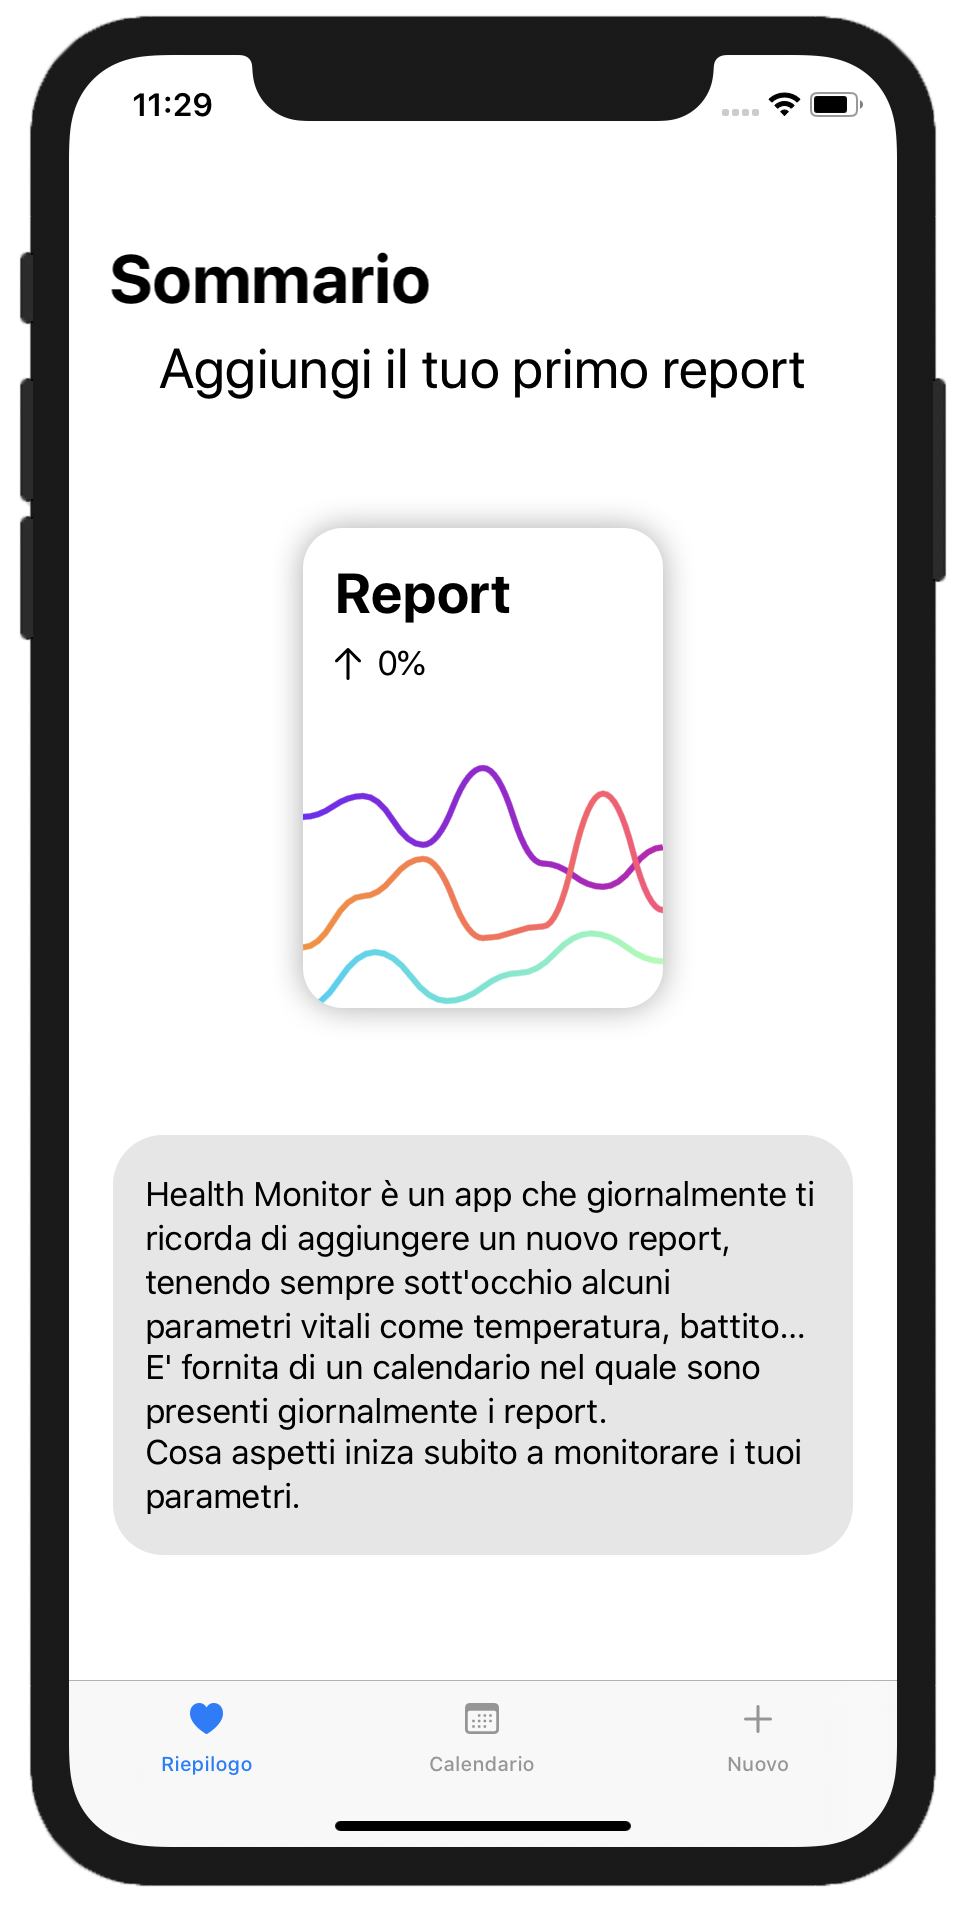
\includegraphics[width=.32\textwidth]{img/riepilogo_iniziale.png}\hfill
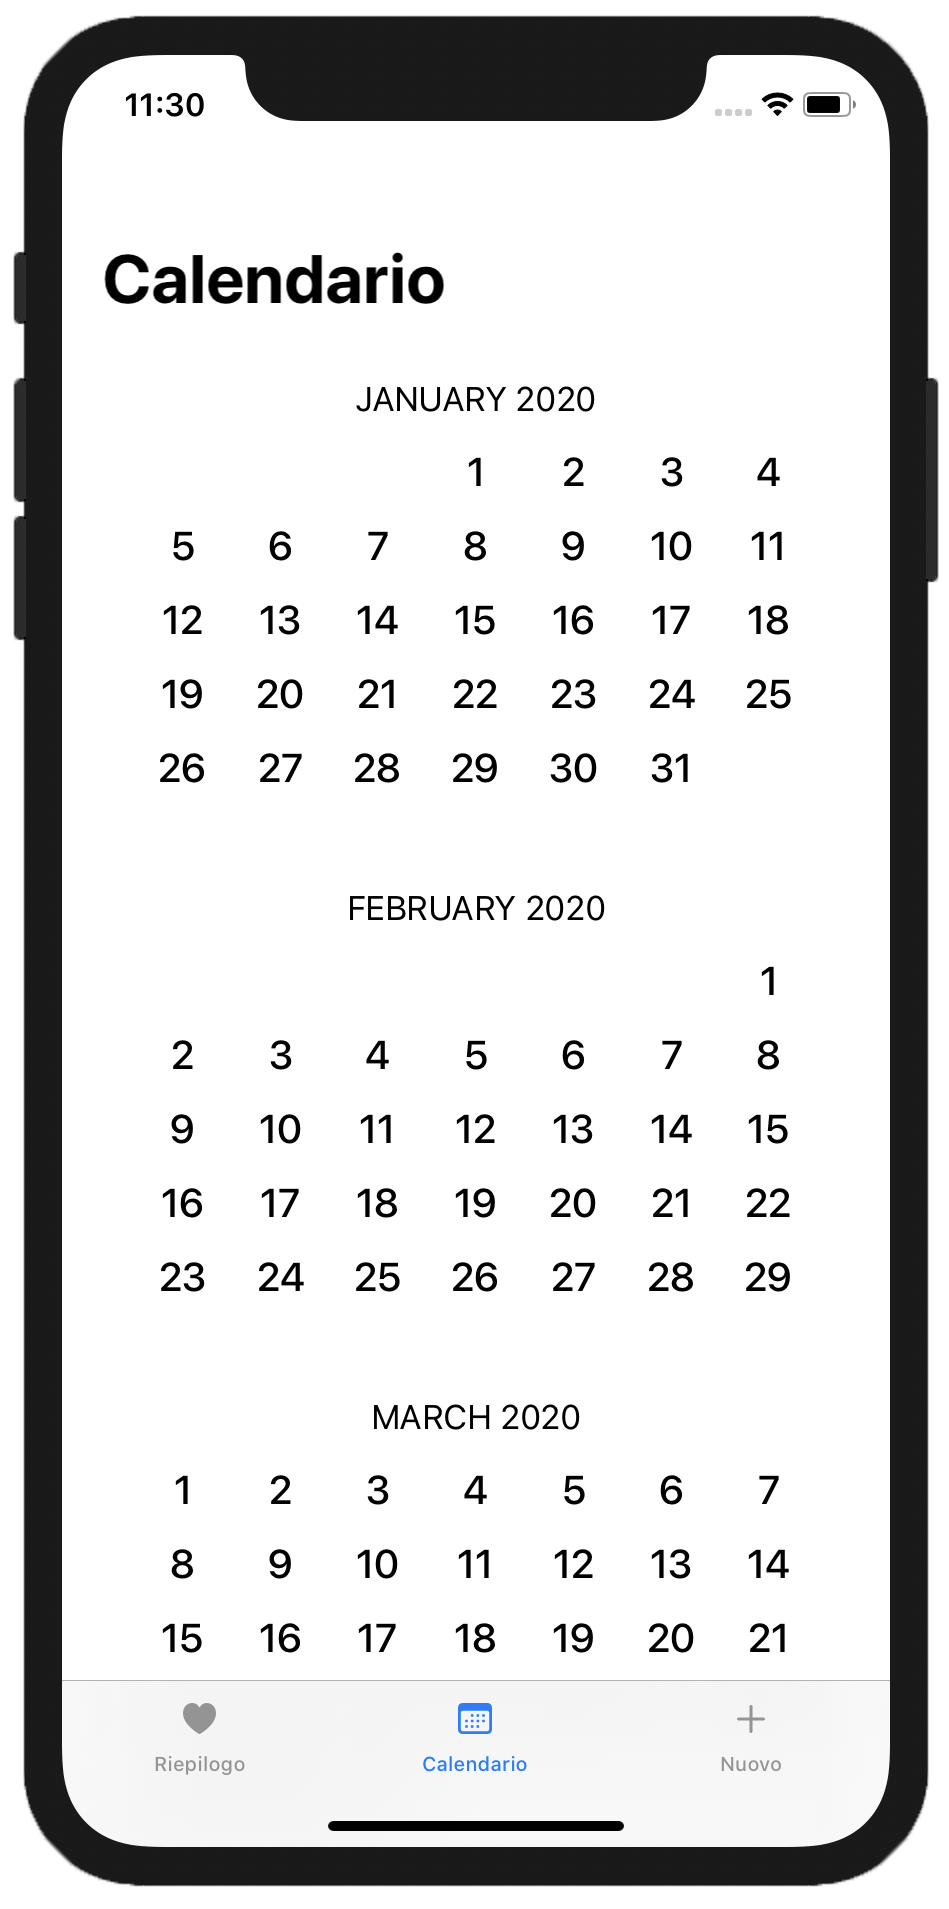
\includegraphics[width=.32\textwidth]{img/calendario_iniziale.png}\hfill
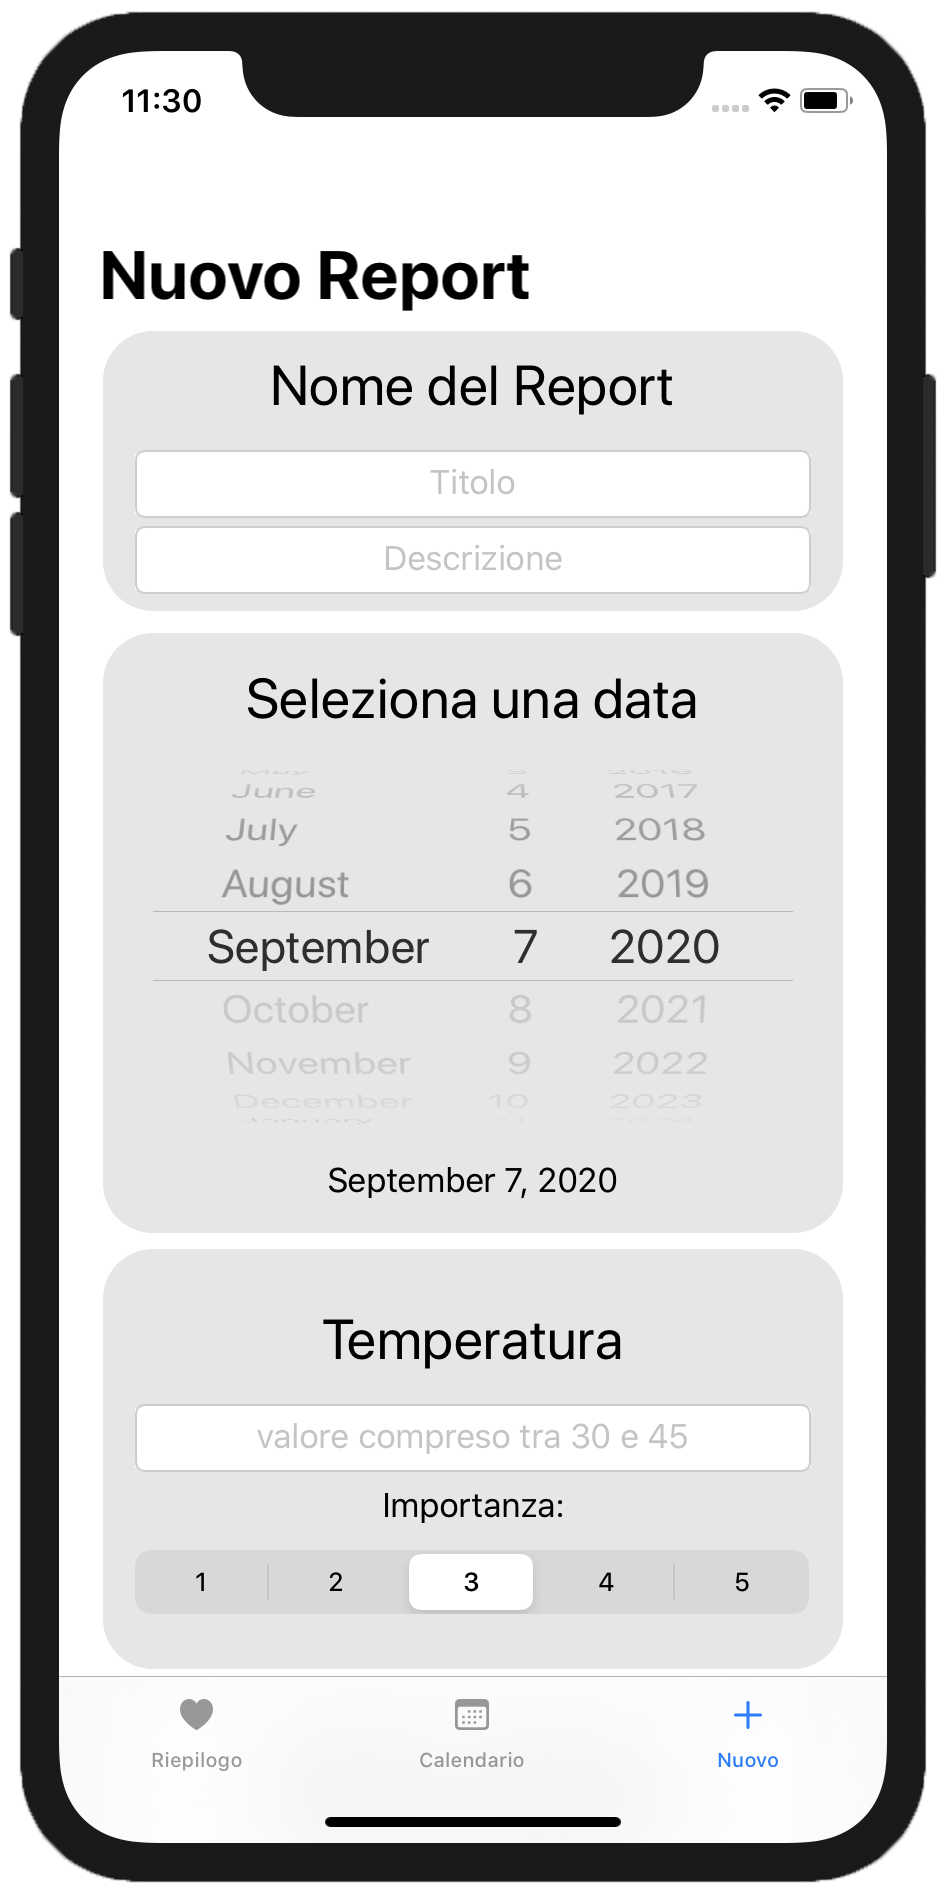
\includegraphics[width=.32\textwidth]{img/nuovo_iniziale.png}

\caption{Schermate Iniziali}
\label{fig:figure1}

\end{figure}

\medskip

\subsection{I Report}

Nella nostra applicazione iOS è possibile aggiungere, modificare ed eliminare dei report giornalieri. \\
I report sono composti da 4 valori e ogni valore ha un importanza che va da 1 a 5. In particolare i valori da inserire possono essere: 
\begin{itemize}
  \item temperatura
  \item battito cardiaco
  \item glicemia
  \item frequenza respiratoria
\end{itemize}

Inoltre ogni report è caratterizzato da una data, un titolo (obbligatori) e una descrizione (facoltativa). 

\subsection{NavigationView}

\begin{figure}[htp]

\centering
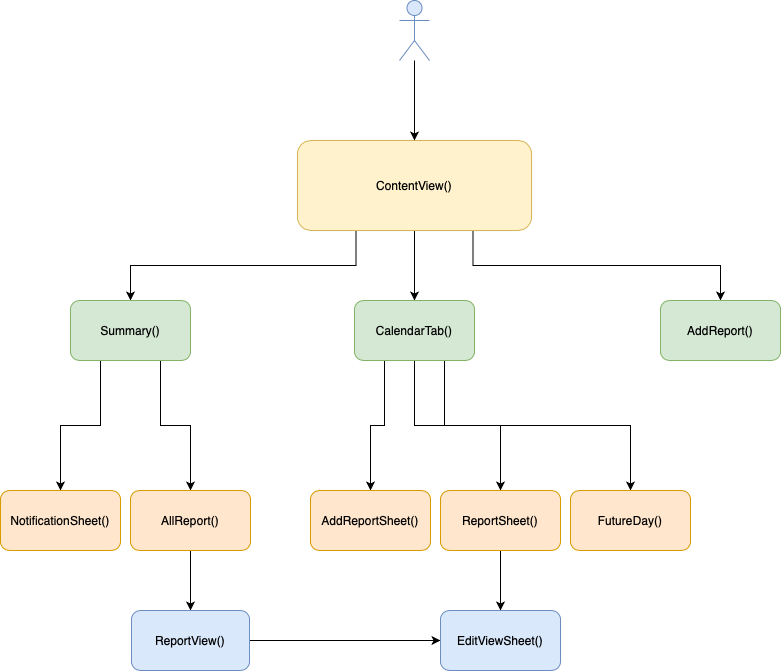
\includegraphics[width=1.1\textwidth]{img/NavigationView.png}\
\label{fig:figure0}

\end{figure}

%----------------------------------------------------------------------------------------
%	Nuovo
%----------------------------------------------------------------------------------------

\newpage
\section{Nuovo}

La Tab "Nuovo" è una delle più importanti per il funzionamento della nostra app. In HealthMonitor vogliamo aggiungere nuovi report quindi questa operazione è stata semplificata il più possibile con una tab specifica. \\
Purtroppo  \textbf{iOS 13} e \textbf{Swift 5} non ci sono venuti incontro quindi diverse funzioni di controllo si sono rese necessarie per la gestione della tastiera. \\
In questa tab si può aggiungere un nuovo report selezionando il giorno sul calendario, e compilando correttamente i campi obbligatori. C'è una funzione di controllo \texttt{validateForm()} che ritorna un Bool, essa ha il compito di sbloccare il tasto "Aggiungi Report" solo quando tutte le voci inserite rispettano i criteri specificati, quindi ritornerà true sse: 
\begin{itemize}
  \item è stato inserito un titolo
  \item è stata inserita una temperatura con un valore tra i 30 ed i 45 gradi
  \item sono stati inseriti il numero di battiti e la glicemia con valori superiori a 40
  \item è stata inserita una frequenza respiratoria con valore superiore a 10 
\end{itemize}
false altrimenti.

\begin{figure}[htp]

\centering
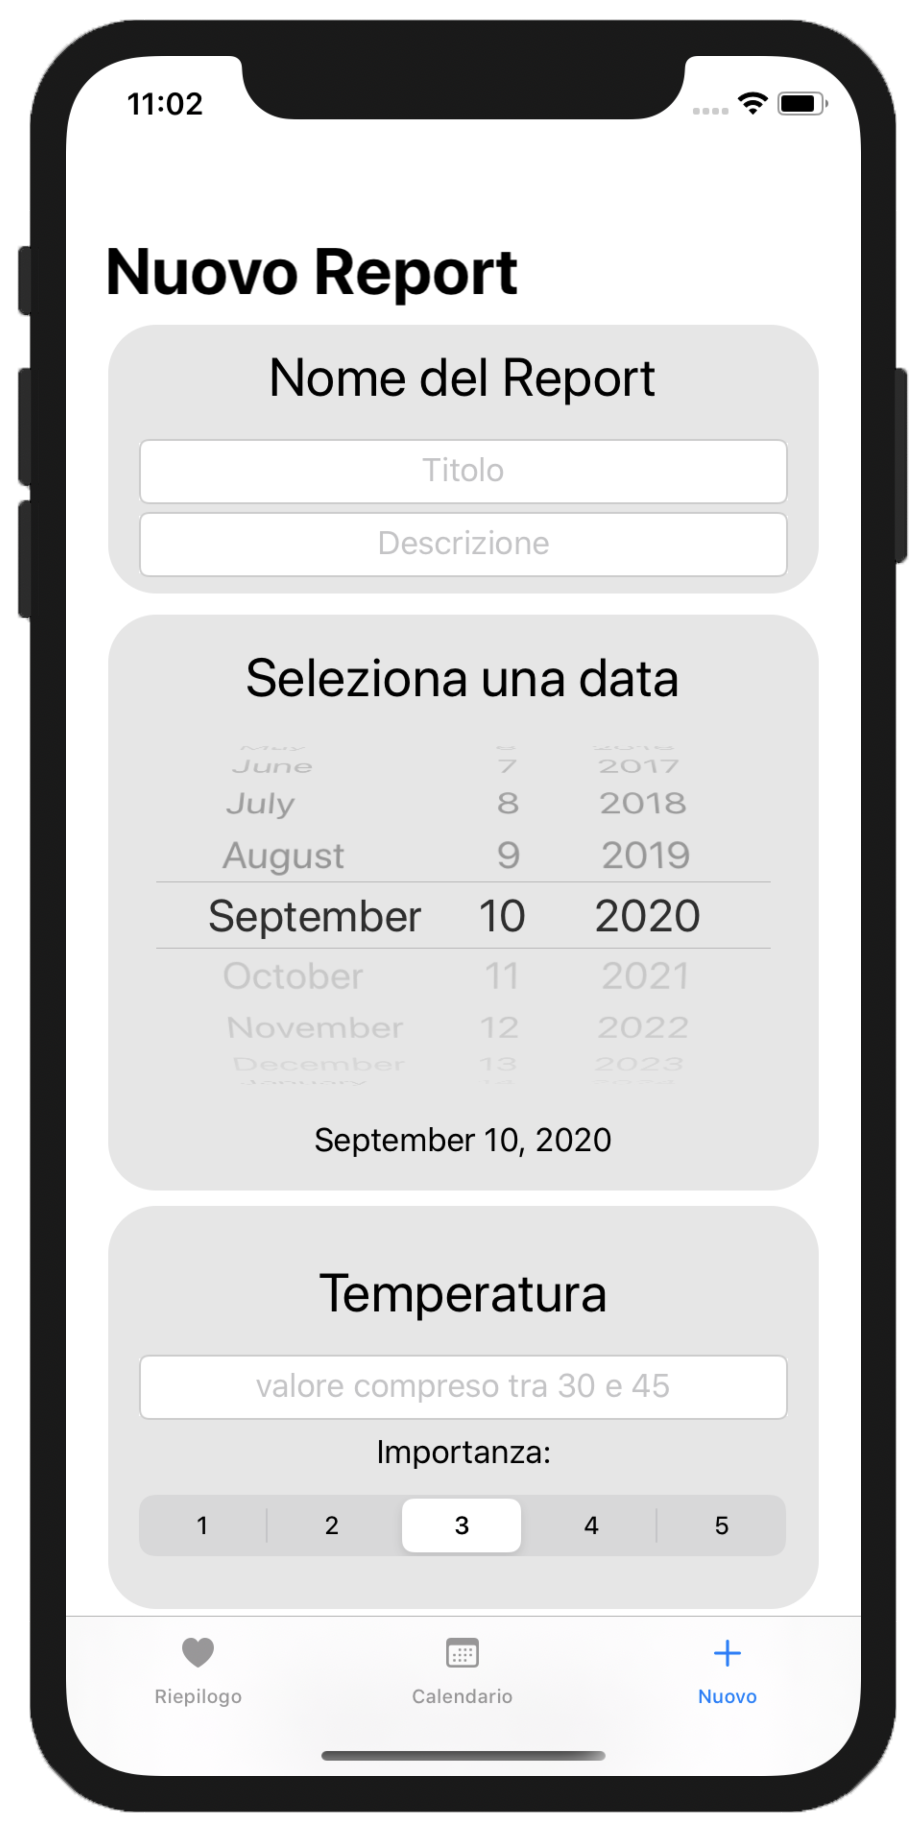
\includegraphics[width=.3\textwidth]{img/nuovo1.png}
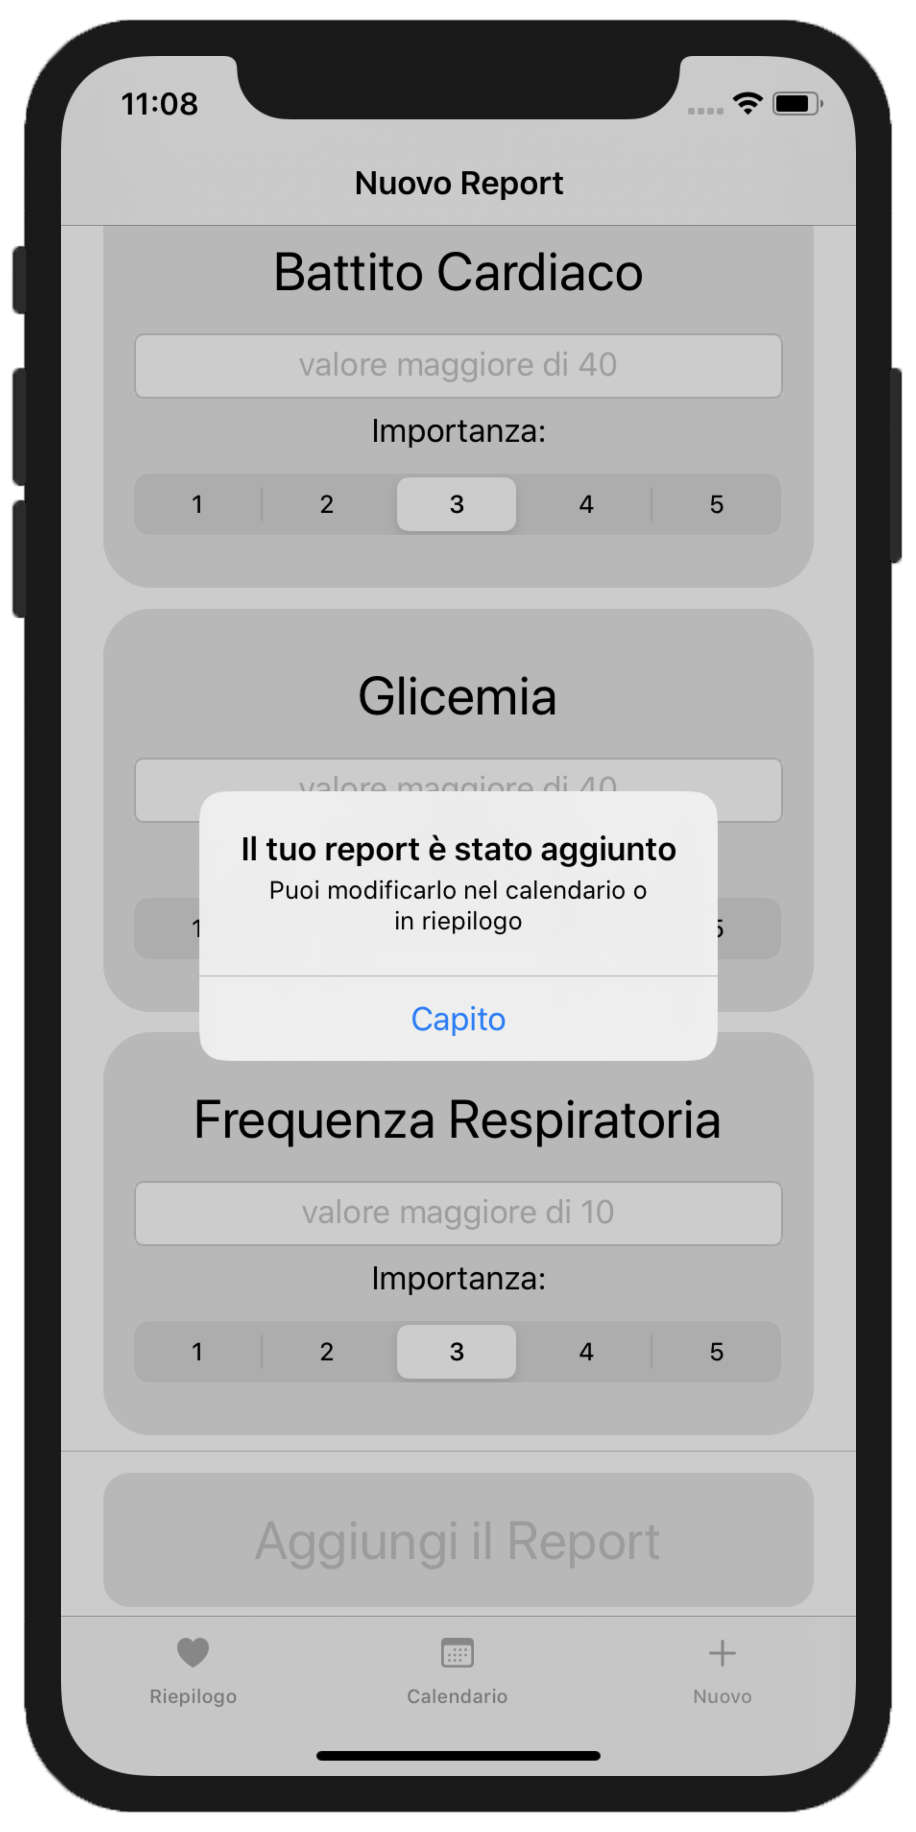
\includegraphics[width=.3\textwidth]{img/nuovo2.png}


\caption{Nuovo report}
\label{fig:figure6}

\end{figure}
\newpage

\subsection{AdaptsKeyboard()}
\begin{wrapfigure}{r}{0.4\textwidth}
  \begin{center}
    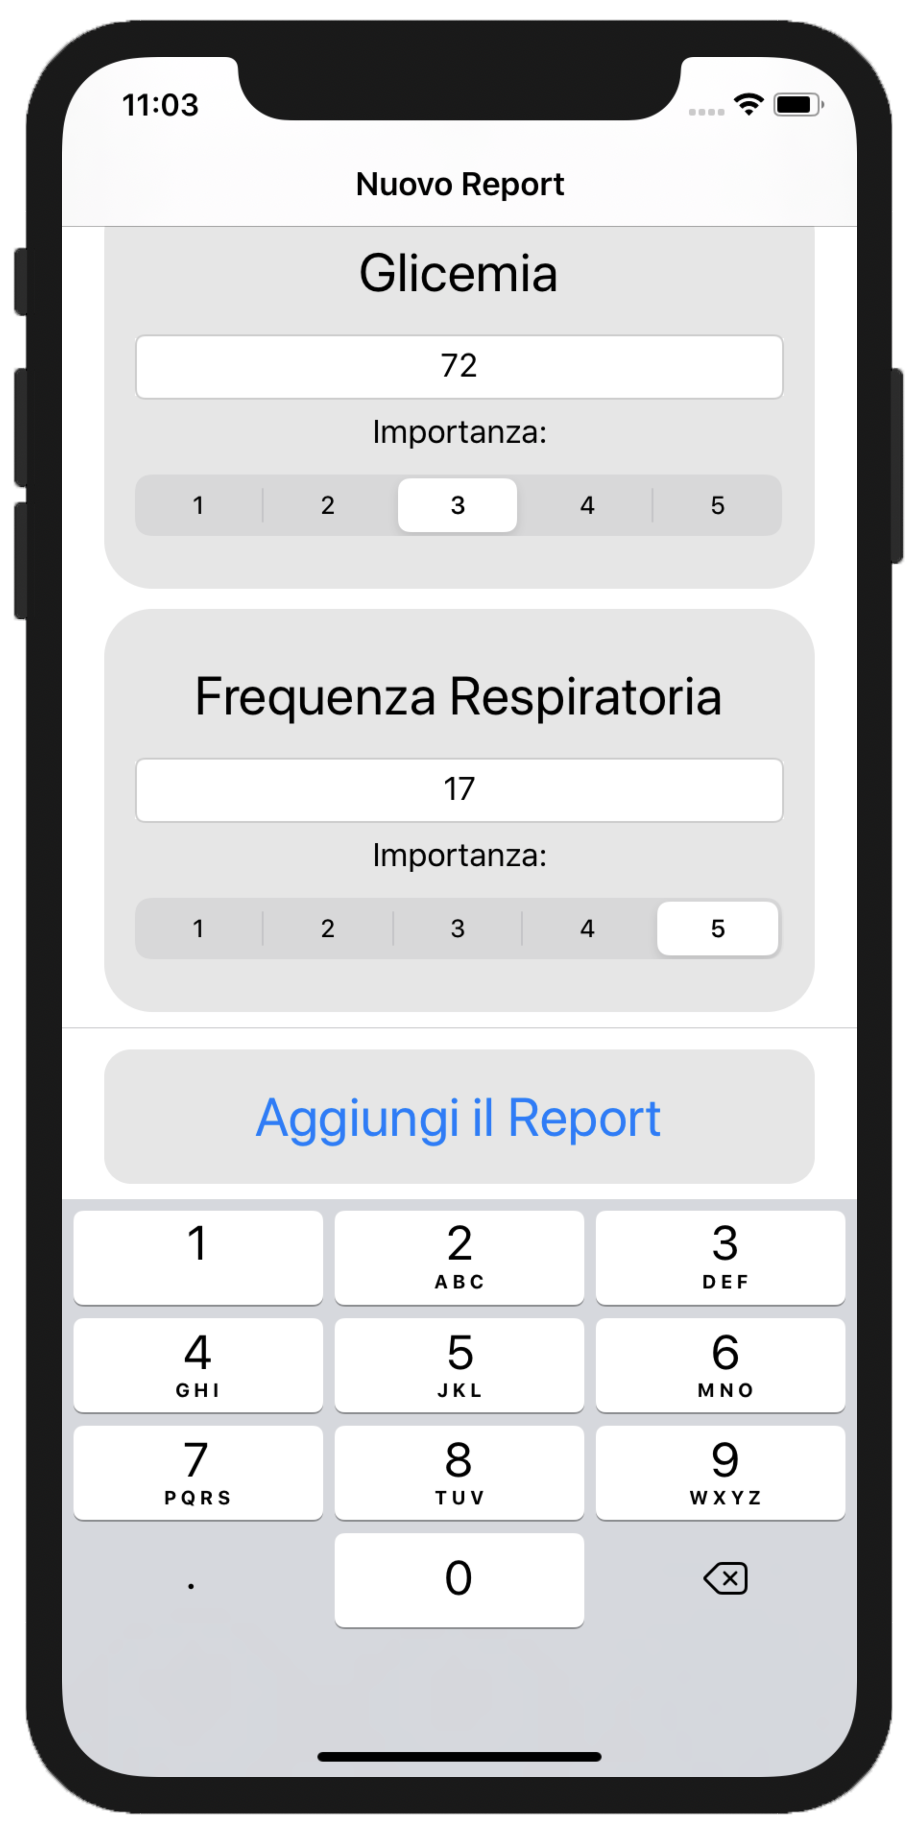
\includegraphics[width=0.3\textwidth]{img/tastiera.png}
  \end{center}
\caption{AdaptsKeyboard()}
\end{wrapfigure}
Per gestire le tastiere sono state scritte due funzioni fondamentali la prima è \texttt{AdaptsKeyboard()}.\\
Essa, quando vengono toccati dei \texttt{TextField}, controlla se la tastiera "copre" il campo dove si dovrebbe scrivere ed in quel caso porta in alto la View appena sopra la tastiera non comprendo con quest'ultima la \texttt{TextField}. Ad esempio quando andiamo ad aggiungere la frequenza respiratoria essendo un campo che si trova alla fine del foglio quando salirà la tastiera non sarà più visibile, qui entra in gioco \texttt{AdaptsKeyboard()} che richiamata alla fine della View controlla tutti campi. 

\subsection{endEditing()}

Un altra funzione fondamentale per facilitare l'utilizzo delle tastiera è \texttt{endEditing()}.\\
Questa funzione si occupa di chiudere la tastiera quando si è finito a scrivere. Essa richiamata nella classe \texttt{SceneDelegate} nel quale specifichiamo che se viene toccato due volte di fila lo schermo, la tastiera deve essere chiusa. 


\subsection{Core Data}

I report vengono salvati e mantenuti in memoria attraverso i Core Data. E' stata creata una nuova entità dal nome \texttt{Report} che presenta in essa i 12 attributi necessari per il salvataggio dei dati. 

\begin{figure}[htp]

\centering
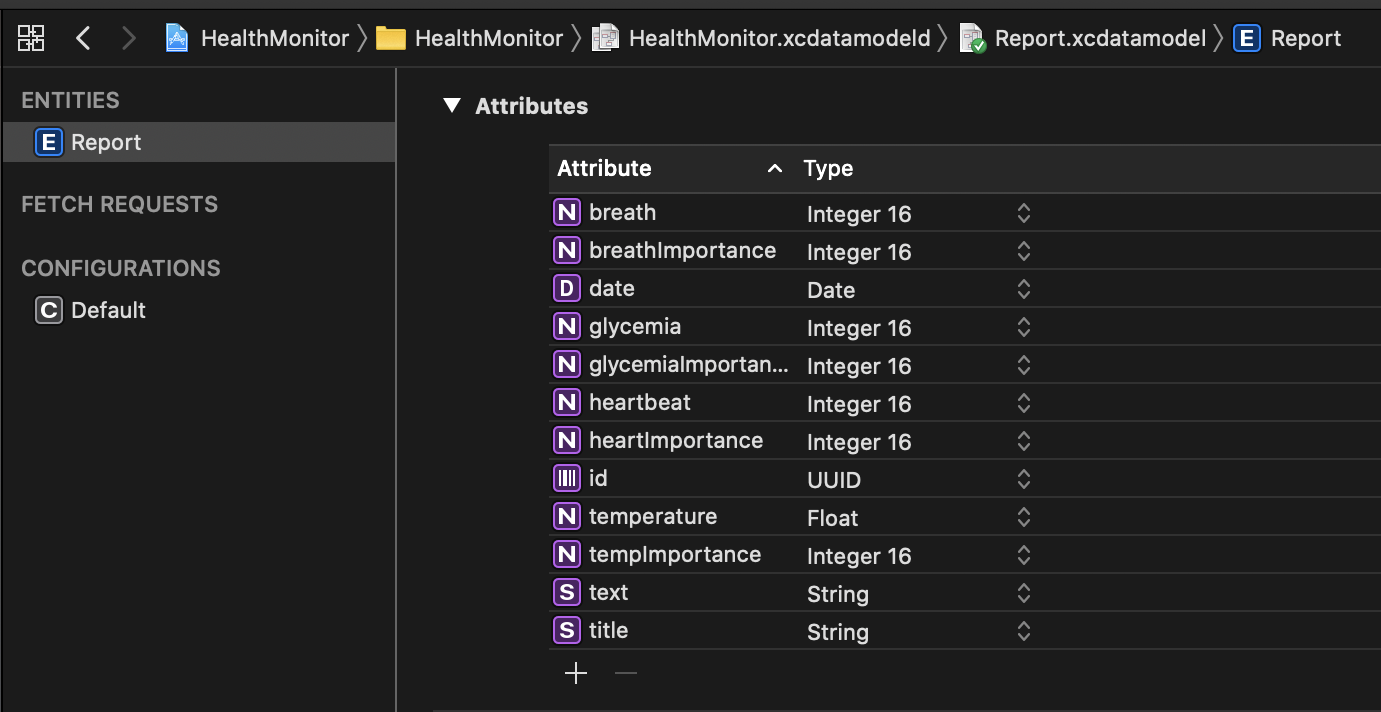
\includegraphics[width=0.9\textwidth]{img/CoreData.png}


\caption{Core Data}
\label{fig:figure6}

\end{figure}

\subsection{Aggiungi un Report}

\begin{lstlisting}
Button(action: {
	self.controlReport()
	self.clearField()
}) {
	ButtonView()
}.disabled(!self.validateForm())
.alert(isPresented: $showingAlert) {
	Alert(title: Text("Il tuo report è stato aggiunto"), message: Text("Puoi modificarlo nel calendario o in riepilogo"), dismissButton: 		.default(Text("Capito")))
}
\end{lstlisting}


Quando viene spinto il pulsante "Aggiungi un report" vengono fatti alcuni controlli prima che il report venga aggiunto. \\
\\
\texttt{controlReport()} si occupa di controllare se il report inserito per quella specifica data è già presente o meno. Se il report è presente verrà calcolata una media tra il report vecchio e quello nuovo, se il report non è presente verrà aggiunto un nuovo report.\\
\\
\texttt{avgReport(report:Report)} è la funzione che, prendendo in input un report calcola la media tra i dati presenti all'interno del report passato come input e i dati che sono stati inseriti nel report, quindi aggiorna il report per quella data con i nuovi dati ed infine salva.\\
\\
\texttt{newReport()} si occupa di creare un nuovo report, inserisce all'interno di ogni campo del Core Data i valori che sono stati messi nel report.\\
\\
\texttt{clearField()} una volta salvato il report, clearField() si occupa di svuotare i \texttt{TextField} dai valori presenti.\\
\\
\texttt{disabled(!self.validateForm())} il bottone risulta diabilitato finche i dati inseriti non sono rispettano i criteri imposti.\\
\\
Infine viene stampato a video un alert che comunica che il report è stato inserito.

%----------------------------------------------------------------------------------------
%	Calendario
%----------------------------------------------------------------------------------------

\newpage
\section{Calendario}

Al centro delle tre \texttt{TabView} troviamo il Calendario che, stilisticamente parlando, è l'oggetto più complesso dell'app.\\
Tramite il calendario possiamo aggiungere eliminare e modificare i report. Inoltre la grafica colorata del calendario ci permette di comprendere i giorni che presentano report ed i giorni senza report. \\
\\
La grafica e la gestione del calendario sono state implementate grazie ad \textbf{\textit{\href{https://github.com/RaffiKian/RKCalendar}{RKCalendar}}}, non trattandosi di una libreria il codice è stato ripulito ed adattato per lo sviluppo di HealthMonitor.\\
Il Calendario è invocato tramite \\
\texttt{CalendarController(reports: self.reports, CalendarManager: self.CalManager)} \\
prendendo in input i report salvati e una classe nel quale sono state inseriti e la data di inizio, di fine calendario ed il tipo di calendario.\\
In CalendarController per ogni mese presente viene richiamata la view \texttt{CalendarMonth()} che è il cuore del nostro calendario, essa non solo si occupa di costruire graficamente il calendario, ma si occupa anche di controllare i giorni e quindi segnalare il giorno corrente, se è presente un report ed il giorno selezionato. I giorni verranno colorati in base a determinate proprietà:
\begin{itemize}
  \item nessun colore $\rightarrow$ nessun report presente $\rightarrow$ è possibile aggiungere un nuovo report
  \item giallo $\rightarrow$ report presente $\rightarrow$ è possibile visualizzare, modificare ed eliminare il report
  \item rosso $\rightarrow$ giorno corrente 
  \item verde $\rightarrow$ giorno selezionato
\end{itemize}

\begin{figure}[htp]

\centering
\includegraphics[width=.3\textwidth]{img/Calendario1.png}\hfill
\includegraphics[width=.3\textwidth]{img/Calendario2.png}\hfill
\includegraphics[width=.3\textwidth]{img/Calendario3.png}

\caption{Calendario con report/Sheet con dettagli report/Sheet con aggiunta report}
\label{fig:figure6}

\end{figure}

\subsection{The sheets}

Nella view "Calendario" non ci spostiamo verso nuove view, ma apriamo solo delle \texttt{sheet}. \\
Come accennato prima il calendario è gestito tutto in \texttt{CalendarMonth()}. Qui troviamo dei controlli fondamentali: 

\begin{lstlisting}
.sheet(isPresented: self.$showSheet) {
	if self.isReport(date: self.CalendarManager.selectedDate ?? Date()) {
		ReportSheet(showSheet: self.$showSheet, reports: self.reports, date: self.CalendarManager.selectedDate)
		.environment(\.managedObjectContext, self.managedObjectContext)
	 }
	 else if (self.CompareDate(date: Date(), referenceDate: self.CalendarManager.selectedDate!)) {
		AddReportSheet(showSheet: self.$showSheet, date: self.CalendarManager.selectedDate ?? Date(), reports: self.reports)
		.environment(\.managedObjectContext, self.managedObjectContext)
	} else {
		FutureDay(showSheet: self.$showSheet)
	}
}
\end{lstlisting}

Quando una data viene toccata \texttt{showSheet} diventa true e quindi viene mostrata la sheet in base alle caratteristiche del giorno:\\
\\
\begin{lstlisting}
if self.isReport(date: self.CalendarManager.selectedDate ?? Date())
\end{lstlisting}
Se nel giorno toccato è presente il report allora verrà mostrato \texttt{ReportSheet()} con le informazioni del report presente per quel giorno.\\
In \texttt{ReportSheet()} possiamo, modificare o eliminare il report corrente. Per la modifica del report abbiamo \texttt{EditViewSheet()} che prendendo in input tutti valori del report, li inserisce nei vari \texttt{TextField} e quindi da la possbilità di cambiare i valori e di inserirne dei nuovi.
\\
\begin{lstlisting}
else if (self.CompareDate(date: Date(), referenceDate: self.CalendarManager.selectedDate!))}
\end{lstlisting}
Se il report per quel giorno non è presente allora ci sono due casi, è una data del calendario presente o passata o è una data del calendario futura.\\
Nel caso che è una data del calendario presente o passata si ha la possibilità di aggiungere un nuovo report grazie a \texttt{AddReportSheet()} che è molto simile a \texttt{AddReport()} ma è ripensata per una \texttt{sheet}.\\
Nel caso si tratta di una data futura allora verrà caricato \texttt{FutureDay()}, una sheet semivuota che avvisa che non si possono aggiungere report futuri. 

%----------------------------------------------------------------------------------------
%	Riepilogo
%----------------------------------------------------------------------------------------

\newpage
\section{Riepilogo}

In riepilogo vengono generati i grafici relativi ai dati inseriti giorno per giorno inoltre è presenta una lista dove si possono consultare tutti i Report, essi  possono essere visualizzati tramite alcuni filtri, possono essere modificati ed eliminati.\\
Se non è presente nessun dato viene caricata una schermata iniziale di benvenuto. 

\begin{figure}[htp]

\centering
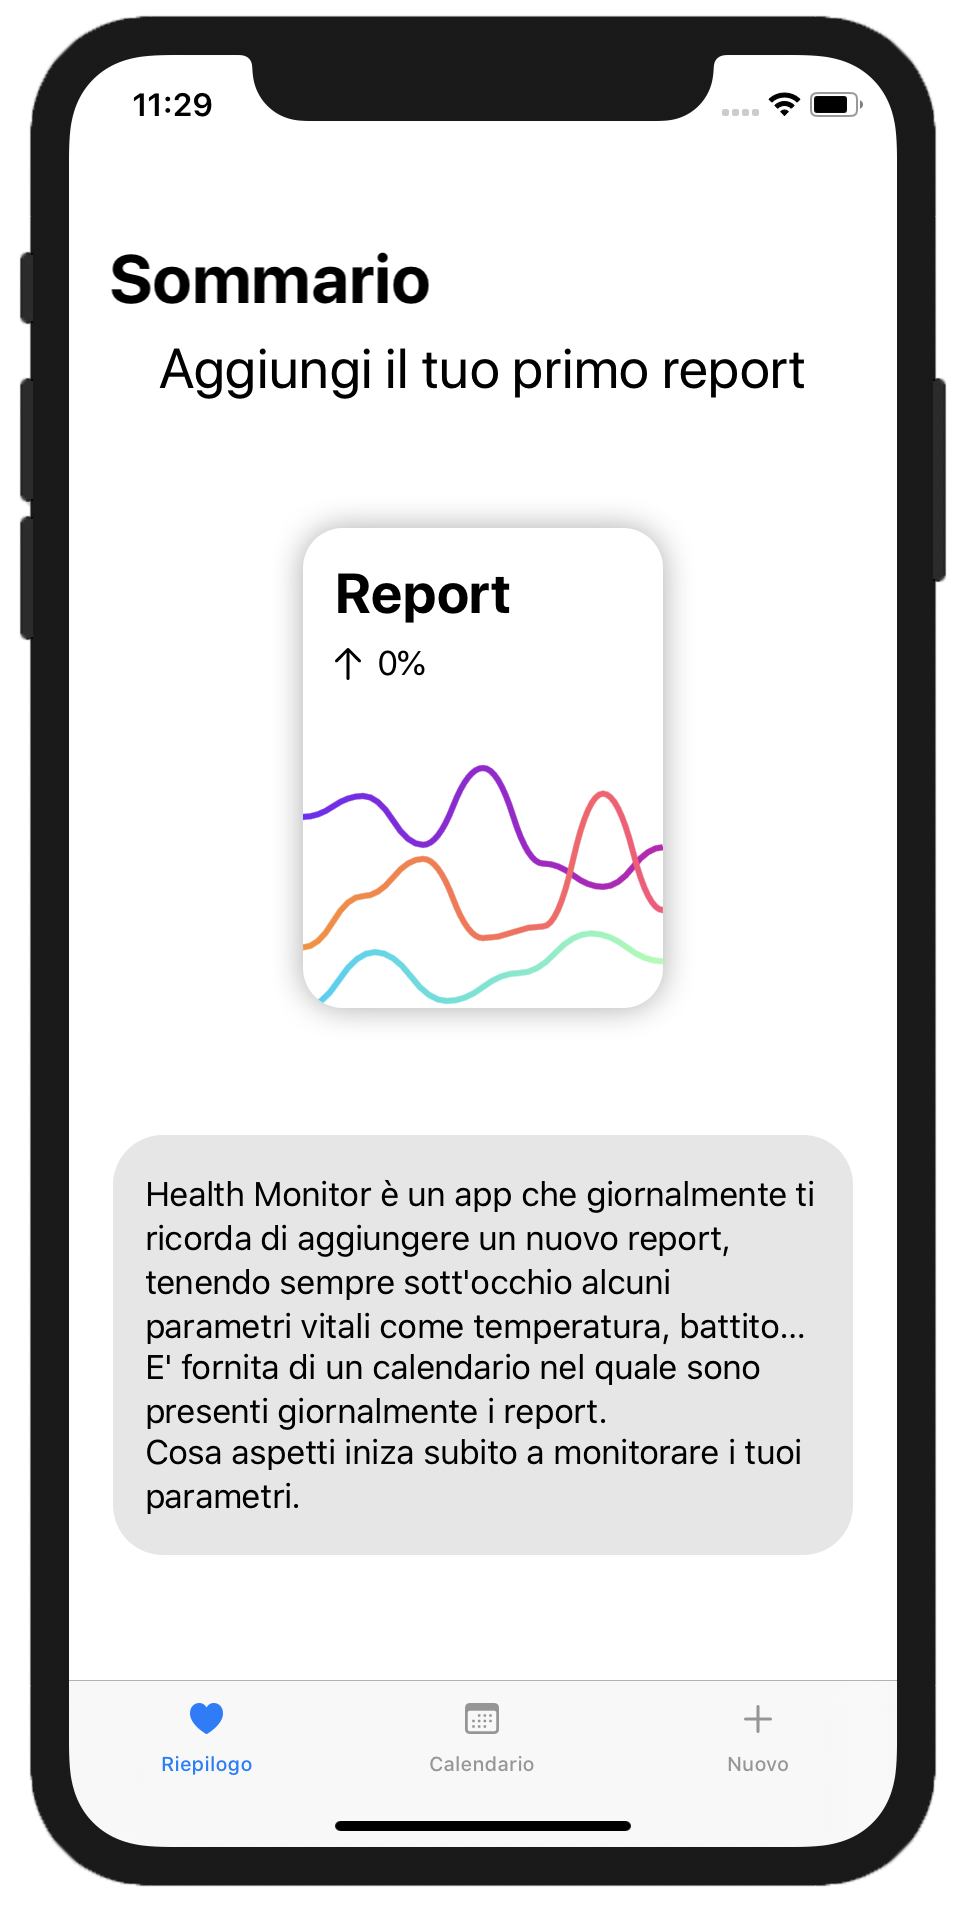
\includegraphics[width=.15\textwidth]{img/riepilogo_iniziale.png}

\caption{Schermata di benvenuto}
\label{fig:figure2}
\end{figure}

\subsection{Grafici}

Quando si inseriscono i dati, si iniziano a generare 4 grafici uno per ogni valore presente nel Report.\\
I grafici vengono generati usando una libreria Swift dal nome \textbf{\textit{\href{https://github.com/AppPear/ChartView}{SwiftUICharts}}}, esso ha diverse configurazioni, in particolare in HealthMonitor troviamo \texttt{LineChartView()} che prende in input array di dati.\\
I valori dei grafici sono ordinati per data, basta trascinare il dito sopra al grafico per visualizzare i valori. 

\begin{figure}[htp]

\centering
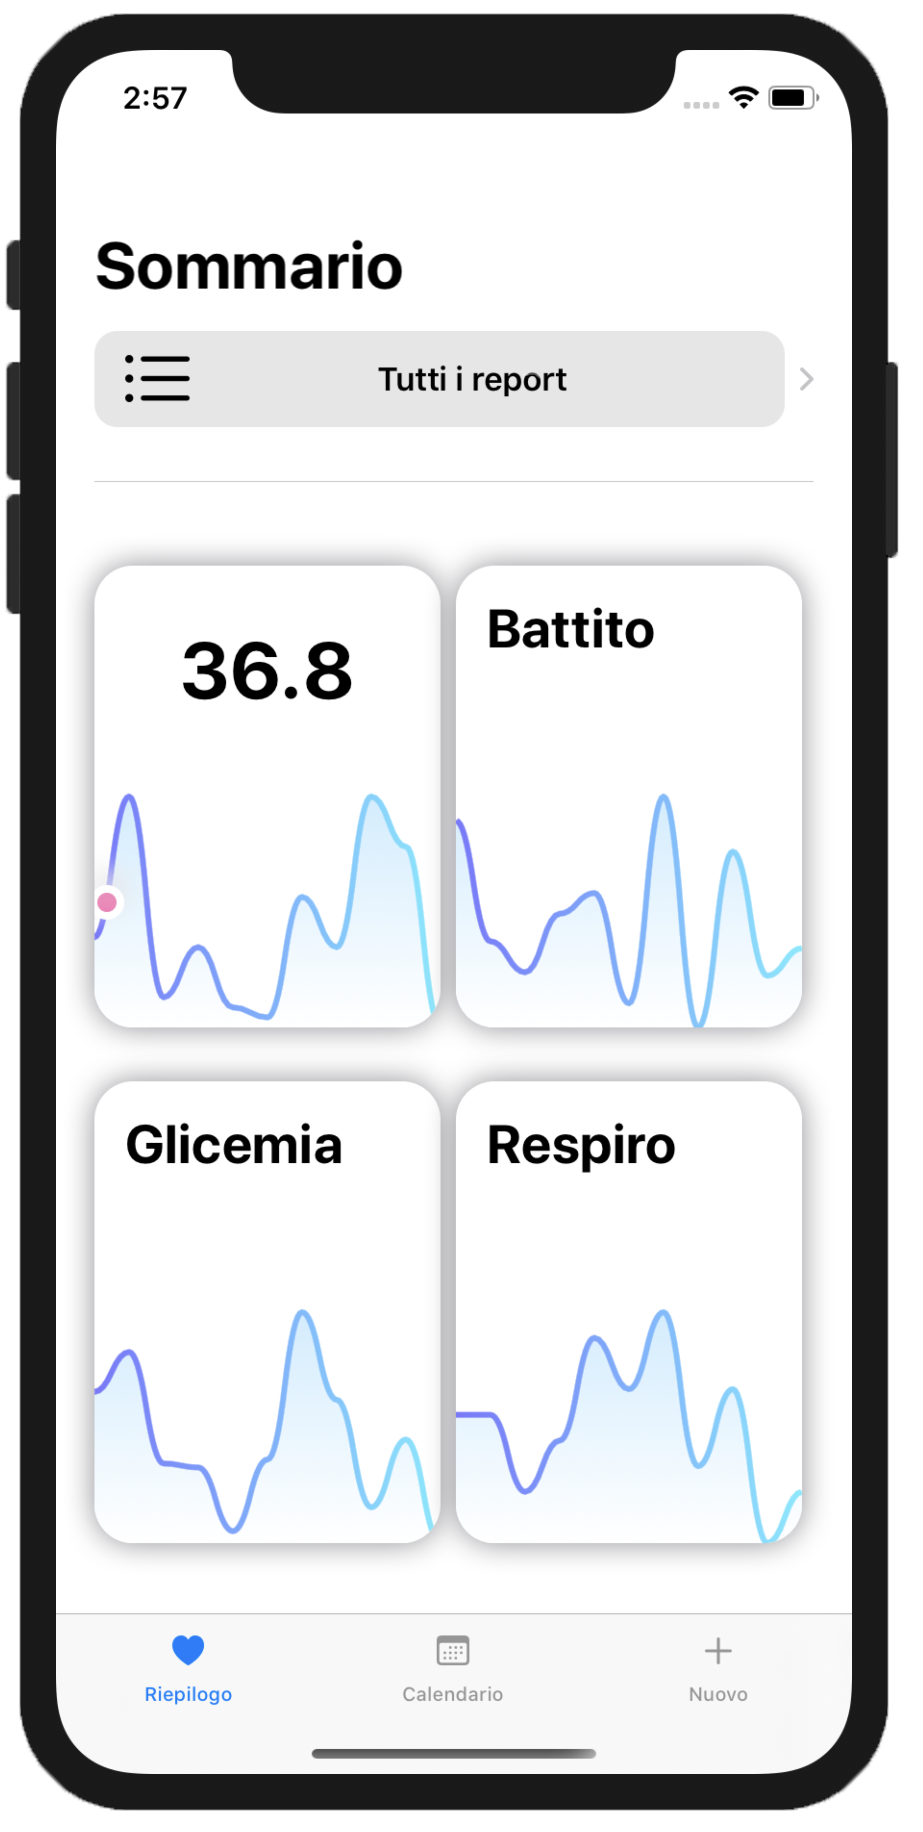
\includegraphics[width=.25\textwidth]{img/grafico1.png}\hfill
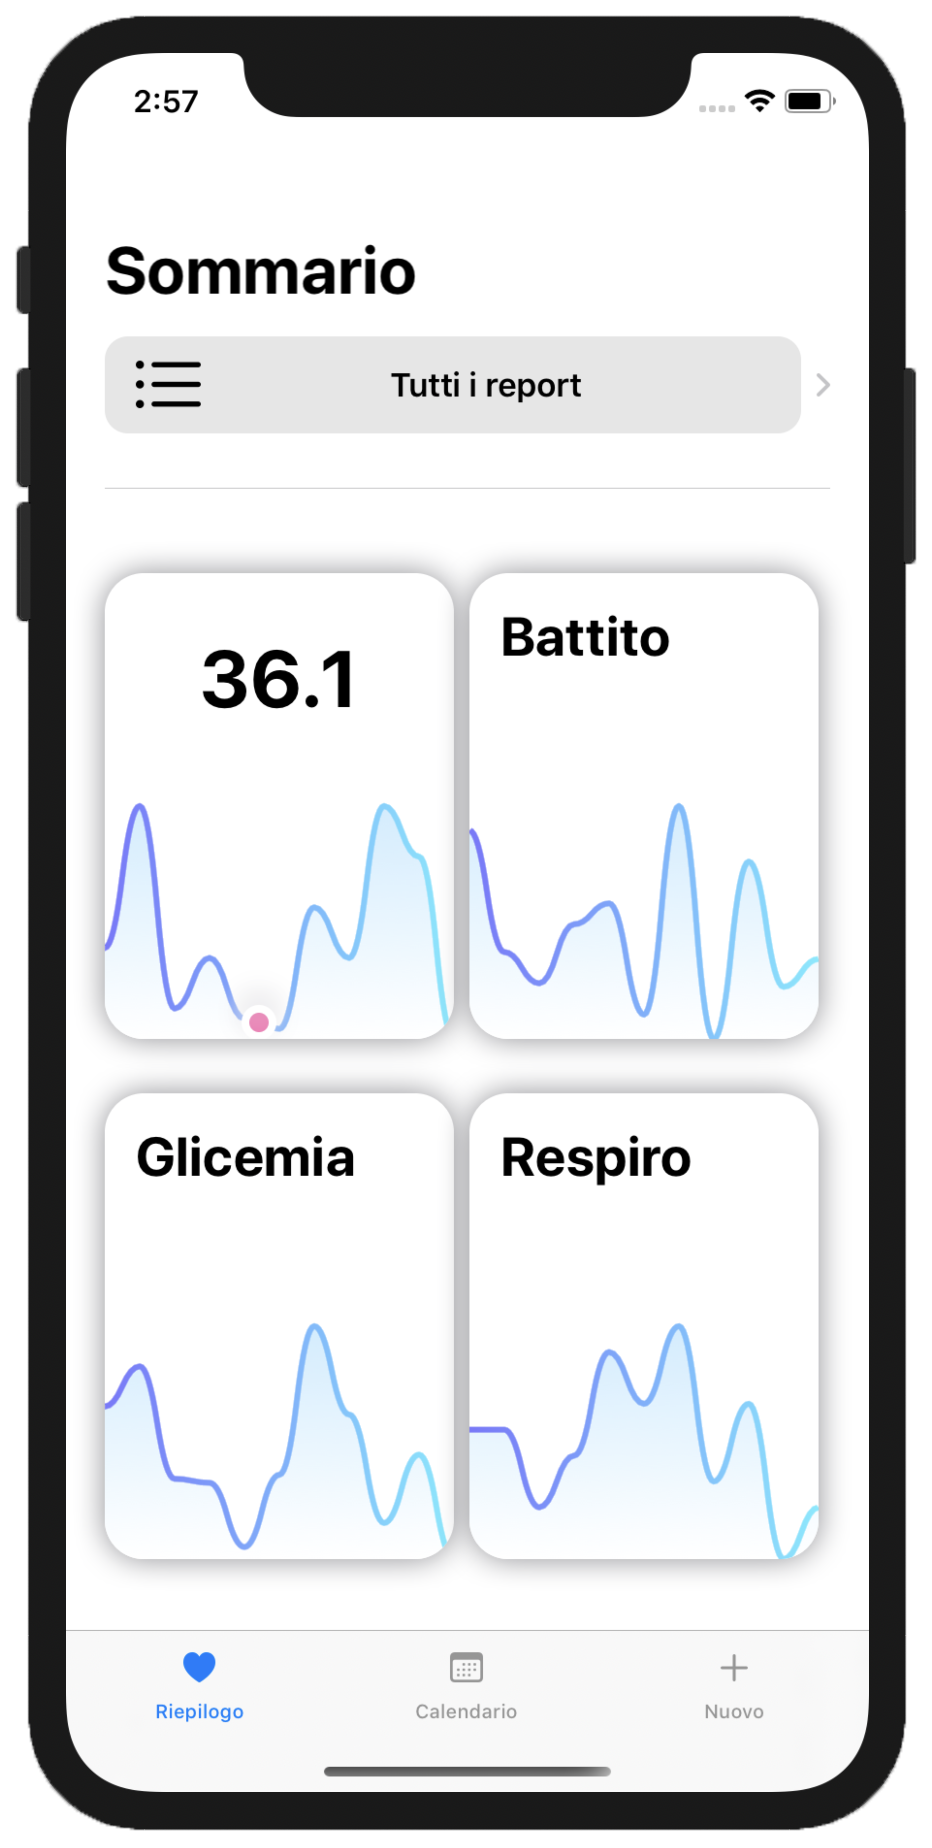
\includegraphics[width=.25\textwidth]{img/grafico2.png}\hfill
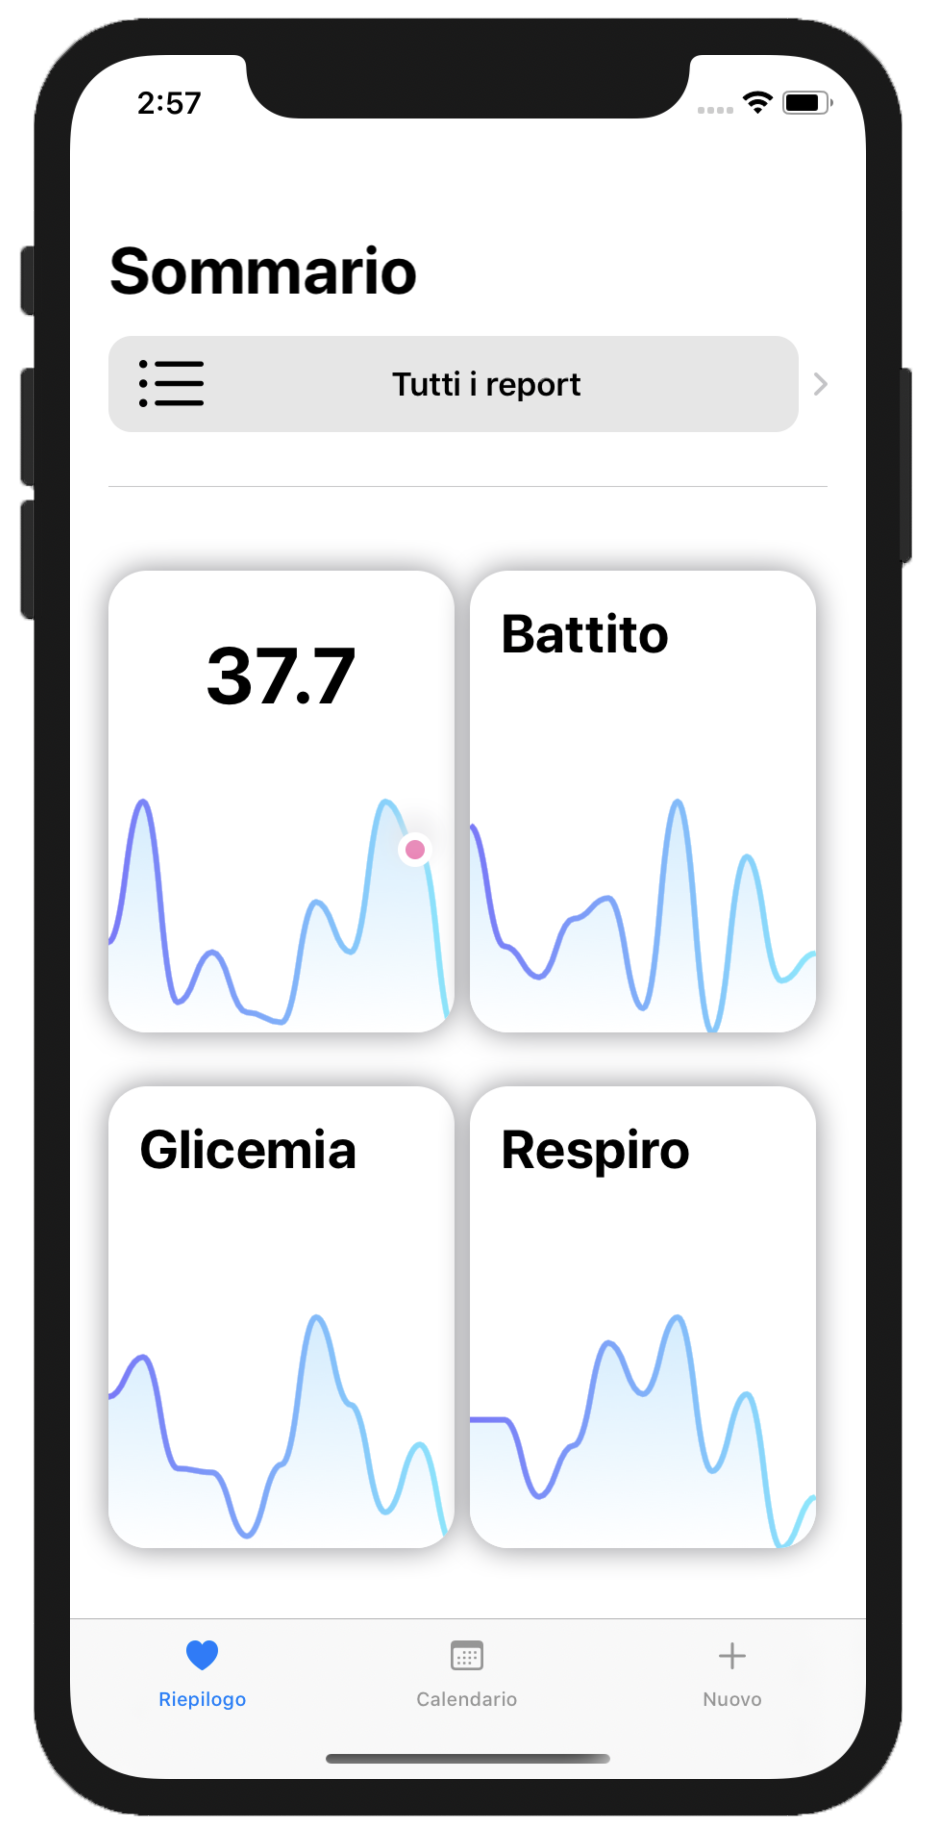
\includegraphics[width=.25\textwidth]{img/grafico3.png}

\caption{Grafici con valori}
\label{fig:figure3}

\end{figure}

\newpage

\subsection{Tutti i Report}

Nella schermata iniziale è presente un \texttt{NavigationLink} che ti permette di spostarti tra le View, toccandoci sopra si caricherà \texttt{AllReport()} nel quale troviamo una lista completa dei Report.

\smallskip

La lista completa dei report in \texttt{AllReport()} è ordinata per data all'interno di una \texttt{List} nel quale ritroviamo i \texttt{NavigationLink} che ci permettono di accedere ai dettagli dei report, inoltre si possono cancellare i report trascinando l'elemento verso sinistra. \\
I report possono essere visualizzati anche tramite dei filtri, che calcolano la media dell'importanza dei 4 valori inseriti e restituisce una lita più corta. La funzione che si occupa del filtraggio dei report è definita nel seguente modo:

\smallskip
\begin{lstlisting}
    private func filterReport() -> [FetchedResults<Report>.Element] {
        return self.reports.filter({
            avgImp(tempImp: $0.tempImportance, heartImp: $0.heartImportance, glyImp: $0.glycemiaImportance, breImpo: $0.breathImportance) >= self.avgImportance
        })
    }
    
    func avgImp(tempImp: Int16, heartImp: Int16, glyImp: Int16, breImpo: Int16) -> Int16 {
        let avgImp : Int16 = (tempImp + heartImp + glyImp + breImpo)/4
        return avgImp
    }
\end{lstlisting}

\begin{figure}[htp]

\centering
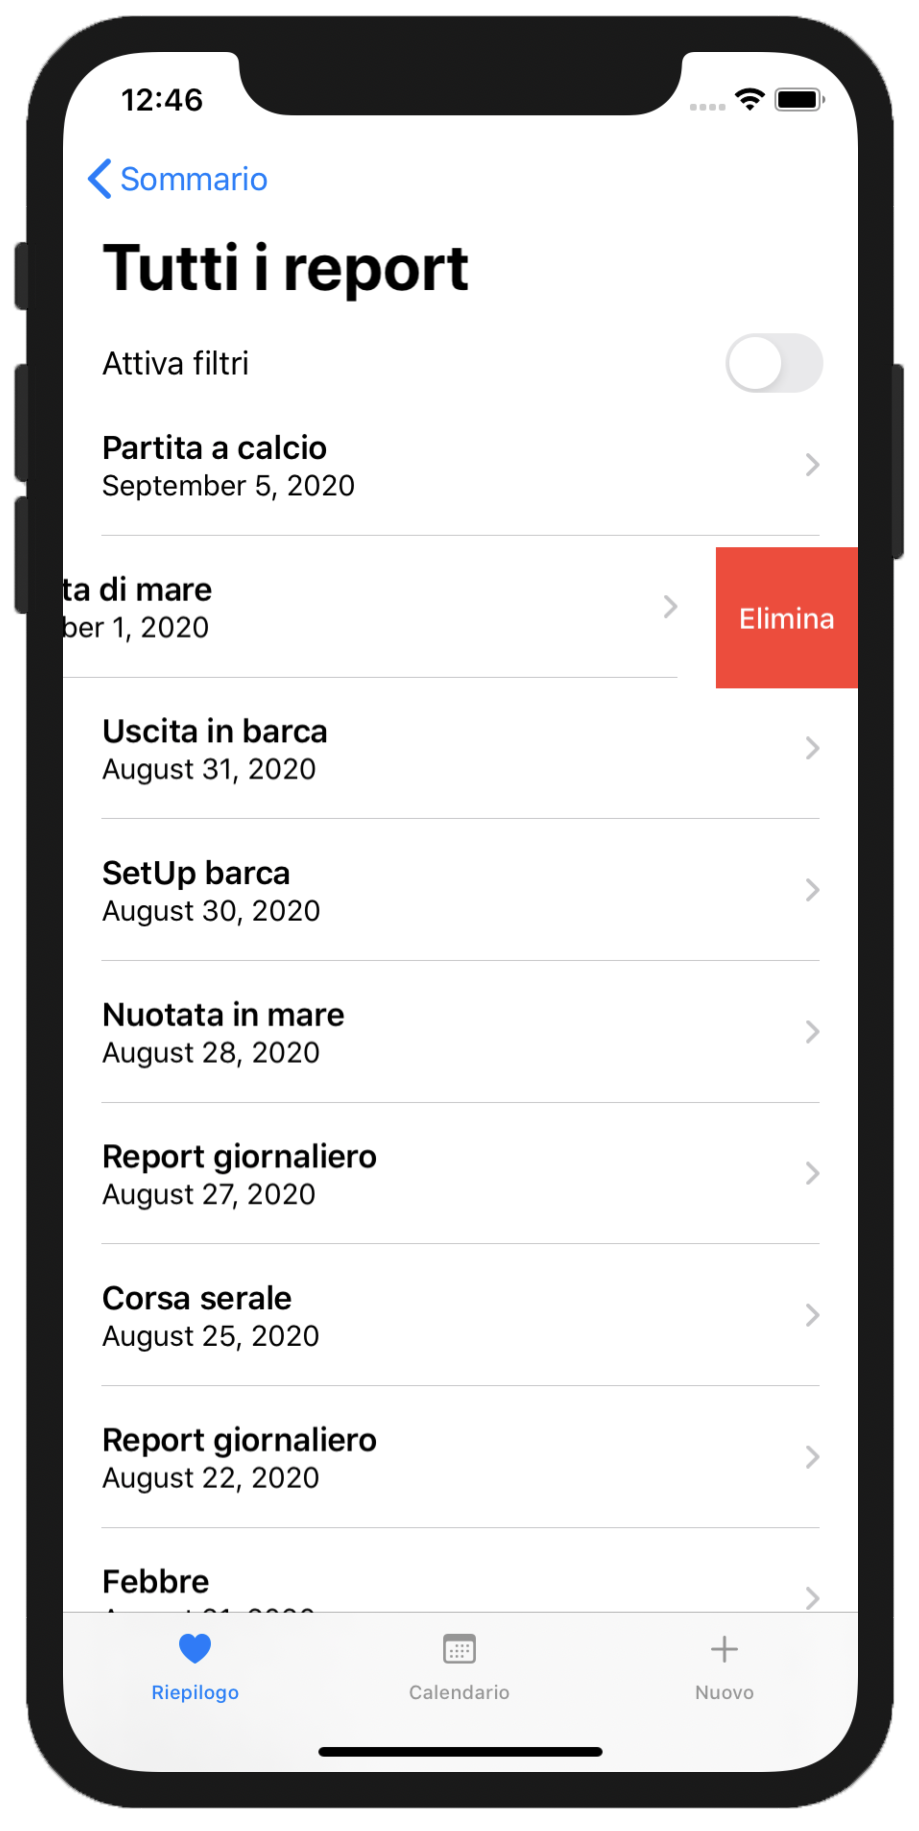
\includegraphics[width=.32\textwidth]{img/tutti1.png}\hfill
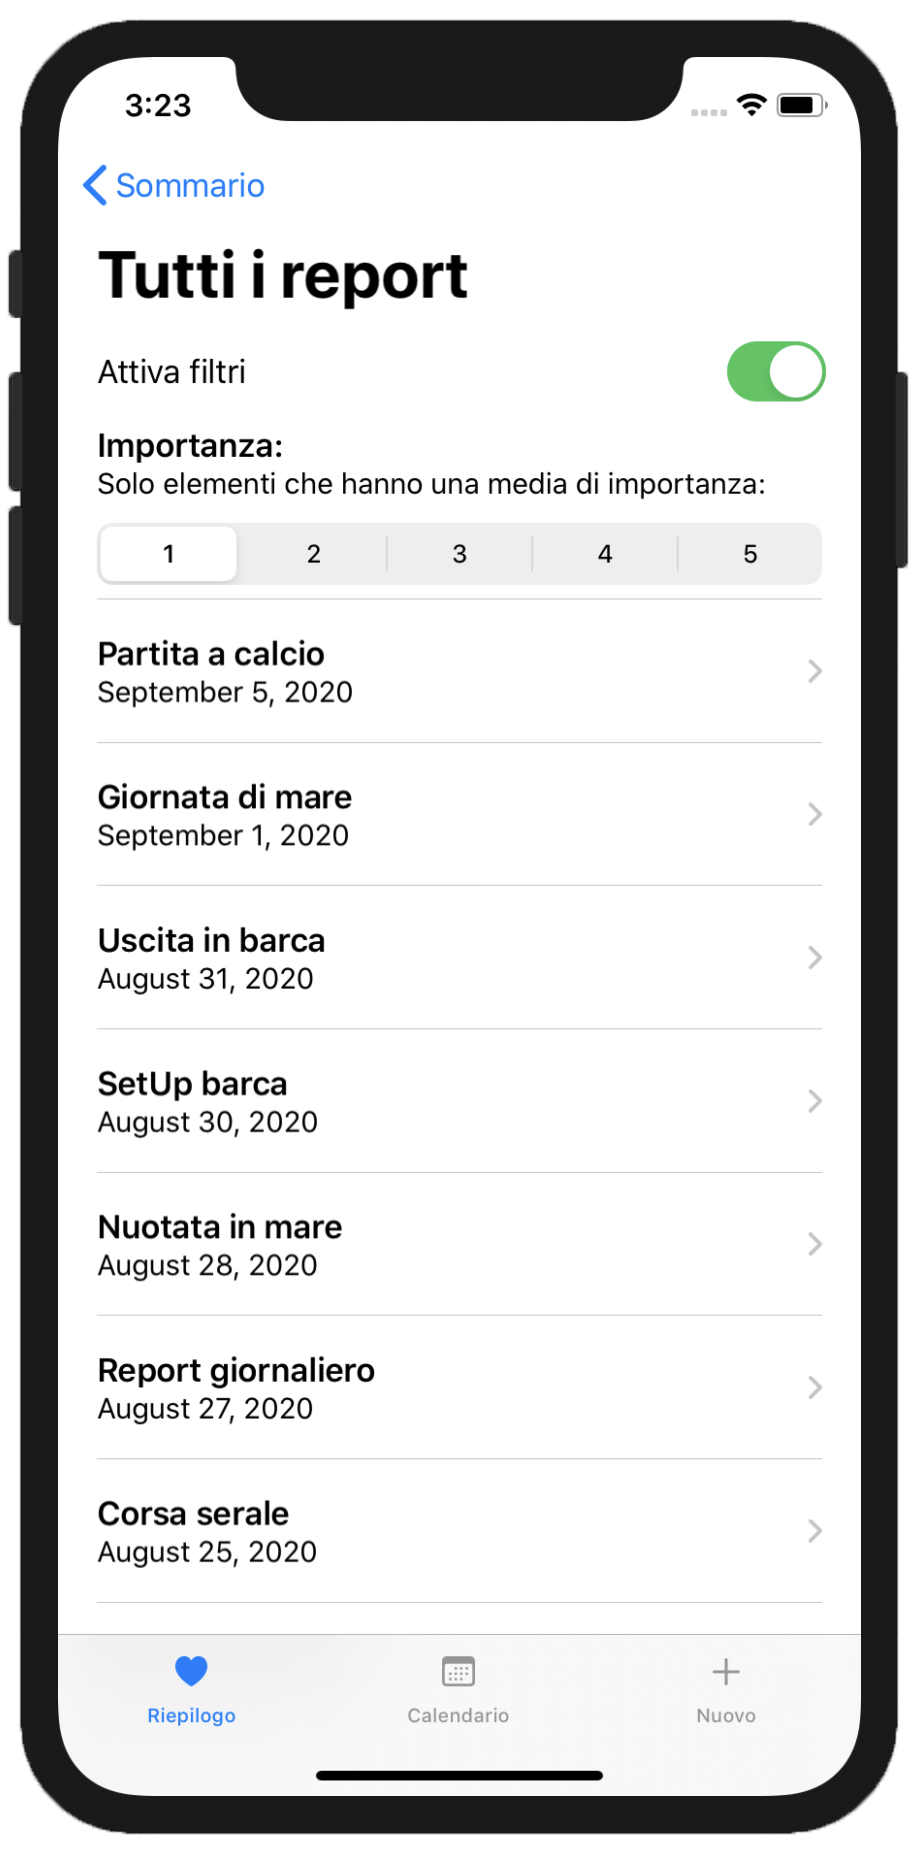
\includegraphics[width=.32\textwidth]{img/tutti2.png}\hfill
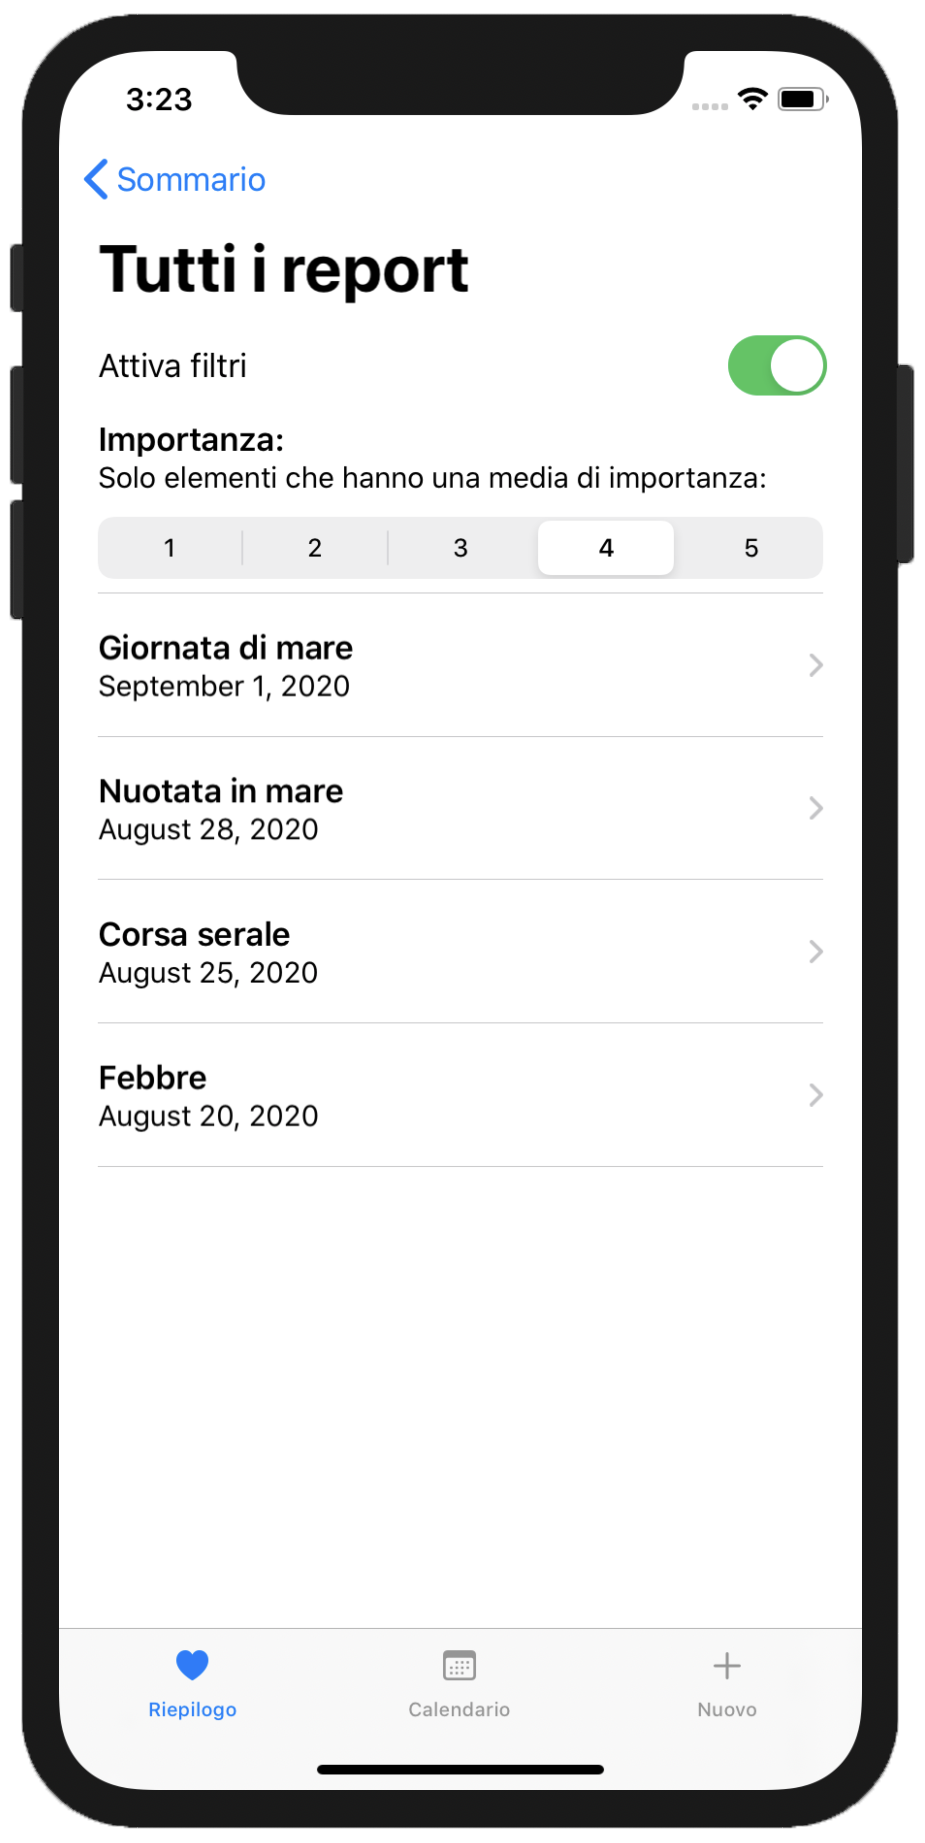
\includegraphics[width=.32\textwidth]{img/tutti3.png}

\caption{Lista Report}
\label{fig:figure4}

\end{figure}

Toccando un oggetto della lista verrà caricata un nuova view \texttt{ReportView()} nel quale troviamo i dettagli del report selezionato. In \texttt{ReportView()}  è possibile modificare il report premendo sul bottone "Modifica il Report", esso caricherà a schermo una nuova \texttt{sheet} e prendendo in input tutti i dati del report corrente verrà mostrato \texttt{EditViewSheet()}. Tramite questa \texttt{sheet} è possibile salvare le modifiche con un bottone a fine pagina, se invece si cambia idea basterà trascinare in basso la \texttt{sheet} o toccare il bottone "Chiudi".

\begin{figure}[htp]

\centering
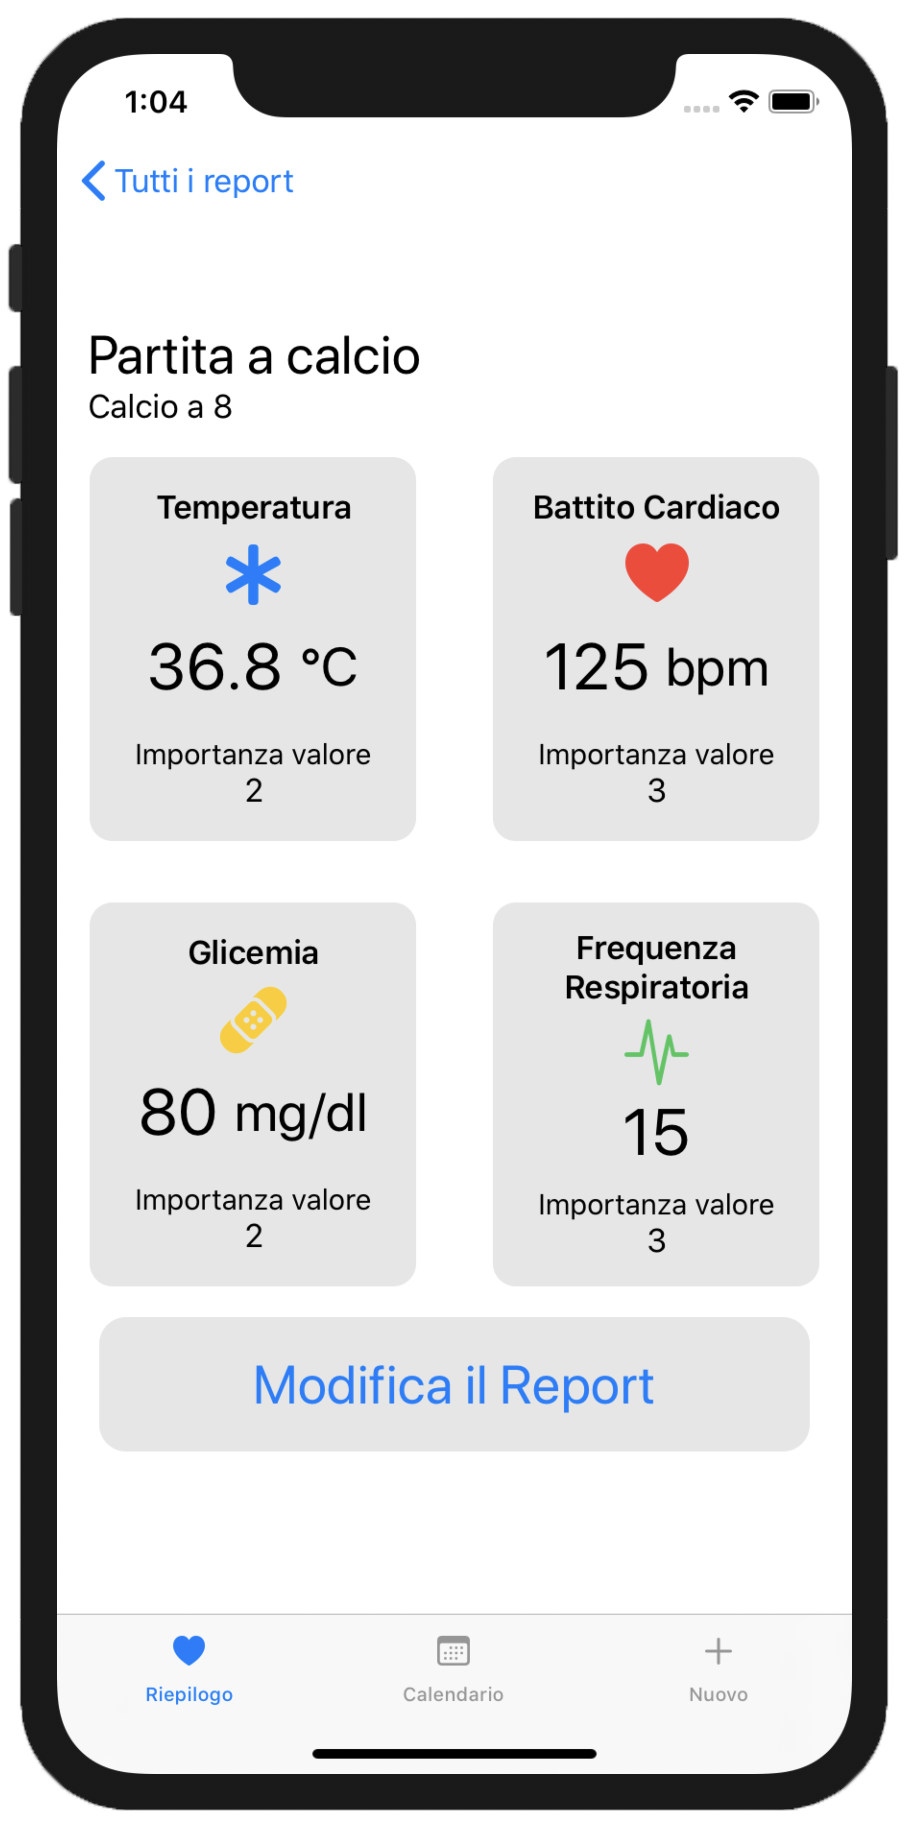
\includegraphics[width=.32\textwidth]{img/ReportView3.png}\hfill
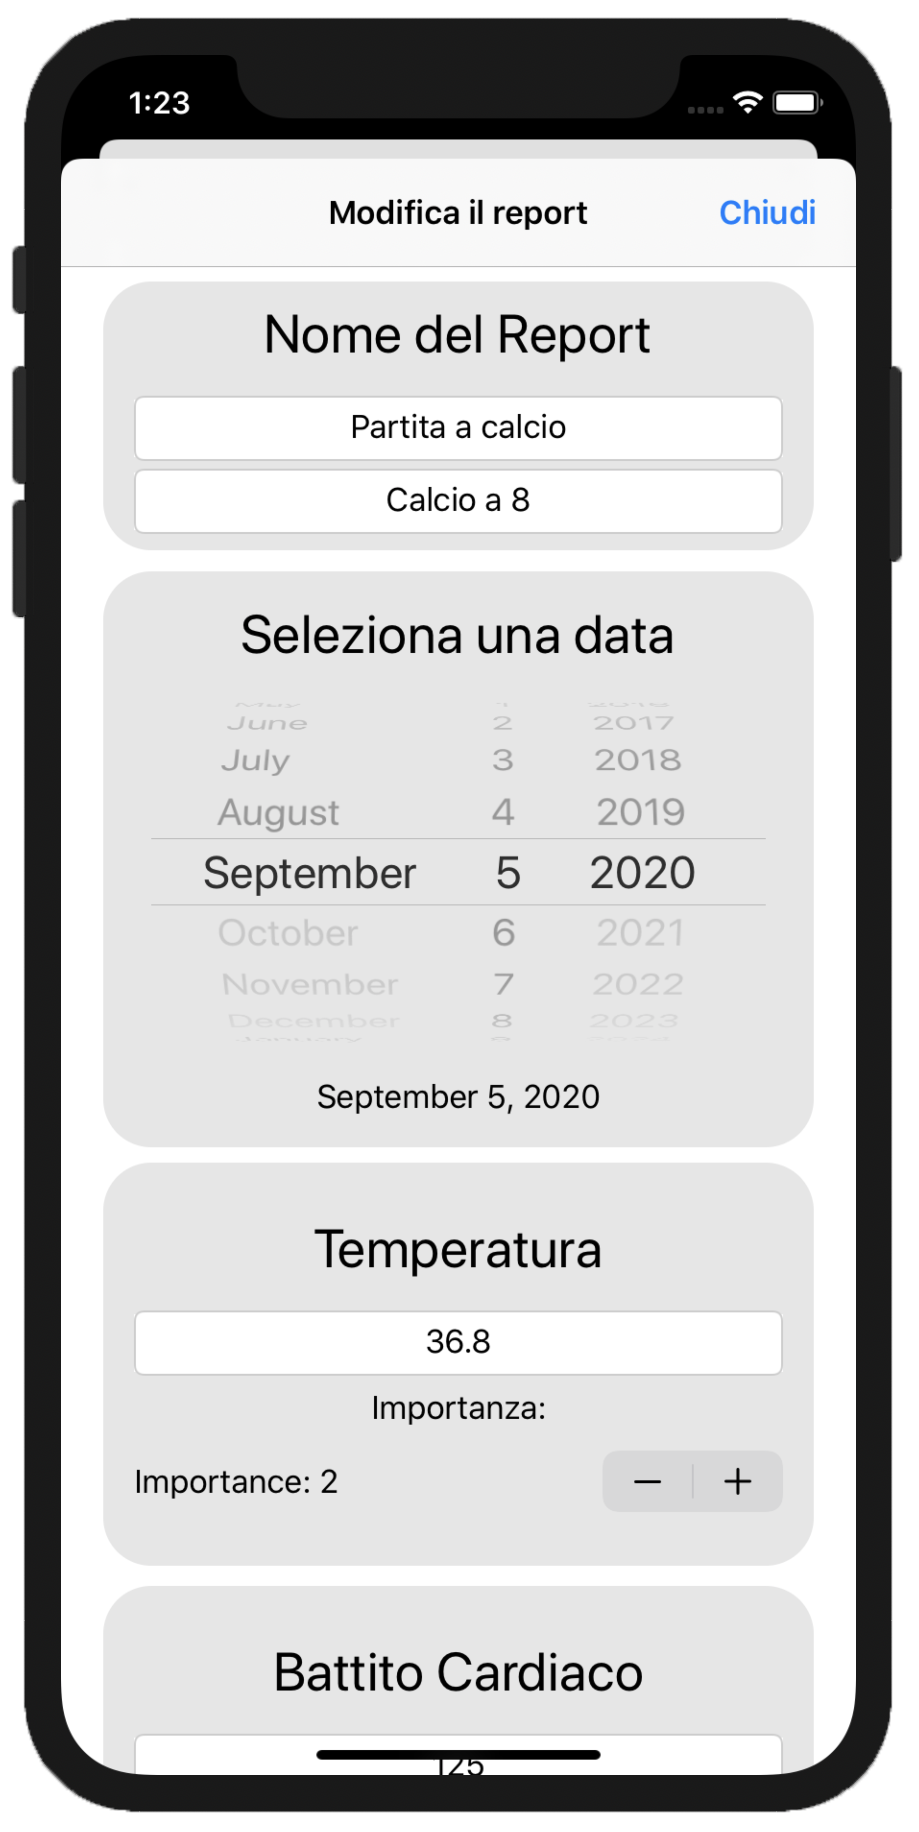
\includegraphics[width=.32\textwidth]{img/ReportView2.png}\hfill
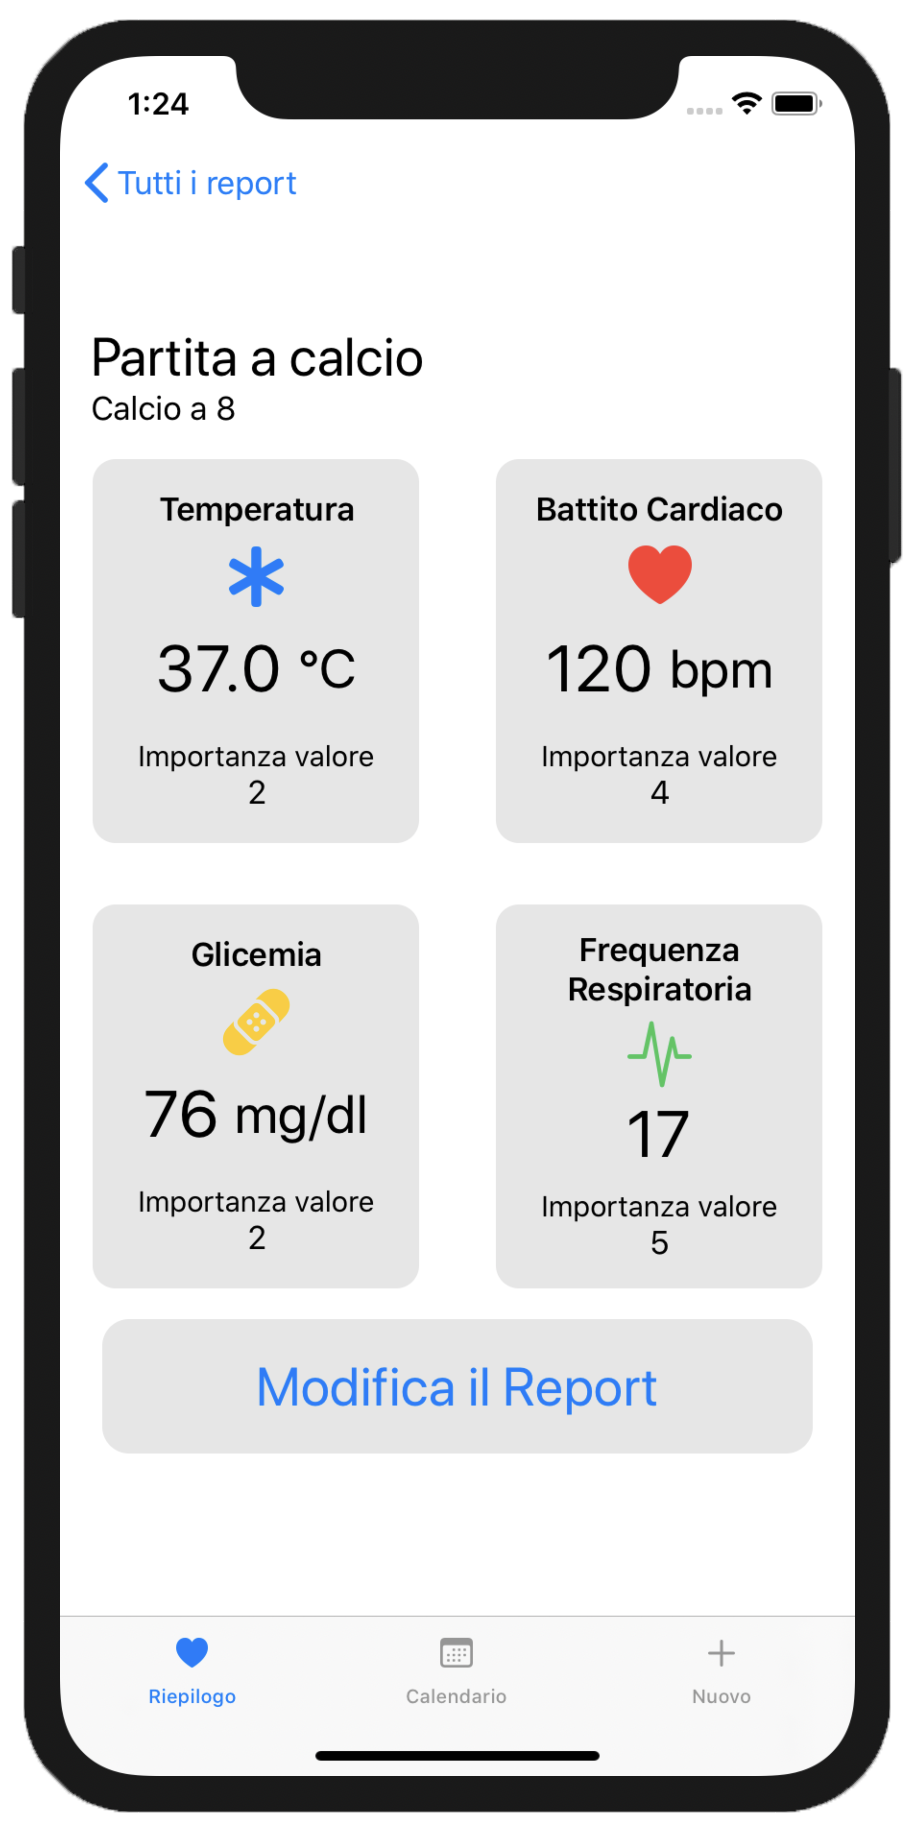
\includegraphics[width=.32\textwidth]{img/ReportView1.png}

\caption{Dettagli del report/Modifica del report/Report modificato}
\label{fig:figure5}

\end{figure}


%----------------------------------------------------------------------------------------
%	Notifiche
%----------------------------------------------------------------------------------------

\newpage
\section{Notifiche}

In HealthMonitor abbiamo la possibilità di ricevere delle notifiche.\\
Le notifiche vengono gestite in \texttt{NotificationSheet()}. Qui si viene avvisati se le notifiche sono attive o disattive. Nel caso sono attive tramite un DatePicker si ha la possbilità di selezionare l'orario in cui si vogliono ricevere le notifiche. Una volta attive le notifiche sono su base giornaliera. Ogni 24h l'app ricorderà all'utente di aggiungere un report. 

\begin{lstlisting}
func sendNotification(start: Date) ->(){
	let content = UNMutableNotificationContent()
	content.title = "Report Giornaliero"
	content.body = "Cosa aspetti? E' giunto il momento di aggiungere il report giornaliero!"
	content.sound = UNNotificationSound.default
        
	var hourStart = DateComponents()
	hourStart.hour = Calendar.current.component(.hour, from: start)
	hourStart.minute = Calendar.current.component(.minute, from: start)
        
	let trigger = UNCalendarNotificationTrigger(dateMatching: hourStart, repeats: true)
	let request = UNNotificationRequest(identifier: "Notification", content: content, trigger: trigger)
	UNUserNotificationCenter.current().add(request, withCompletionHandler: nil)
}    
\end{lstlisting}

\begin{figure}[htp]

\centering
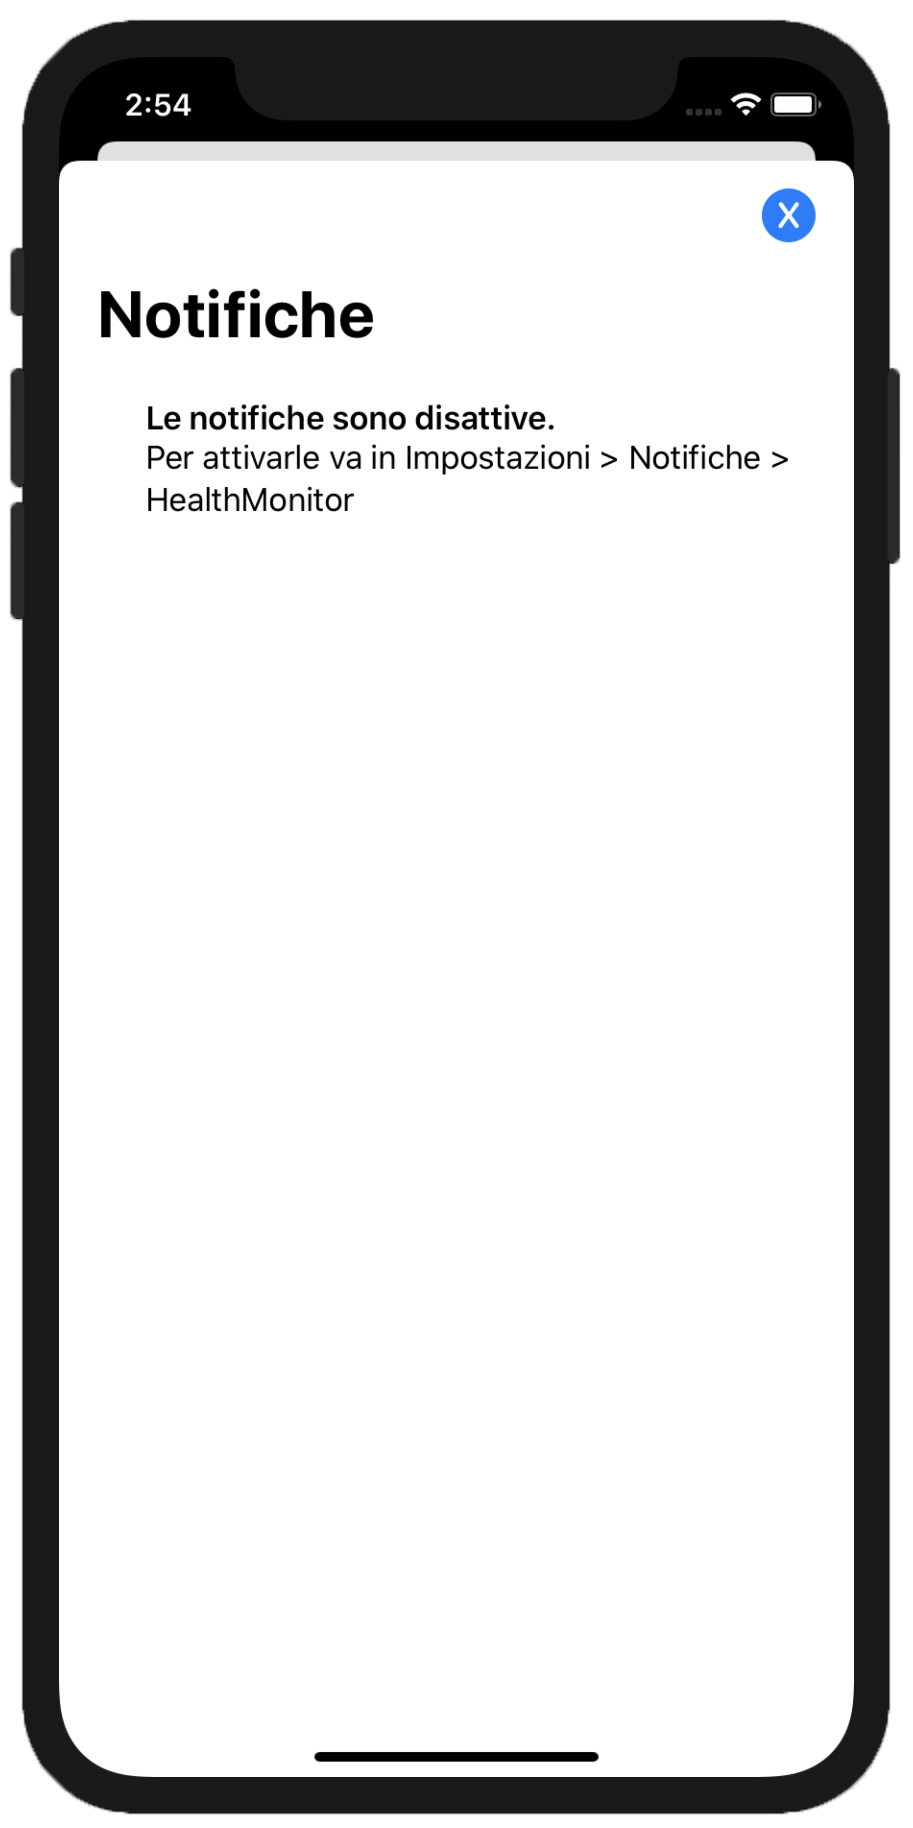
\includegraphics[width=.32\textwidth]{img/notifiche1.png}\hfill
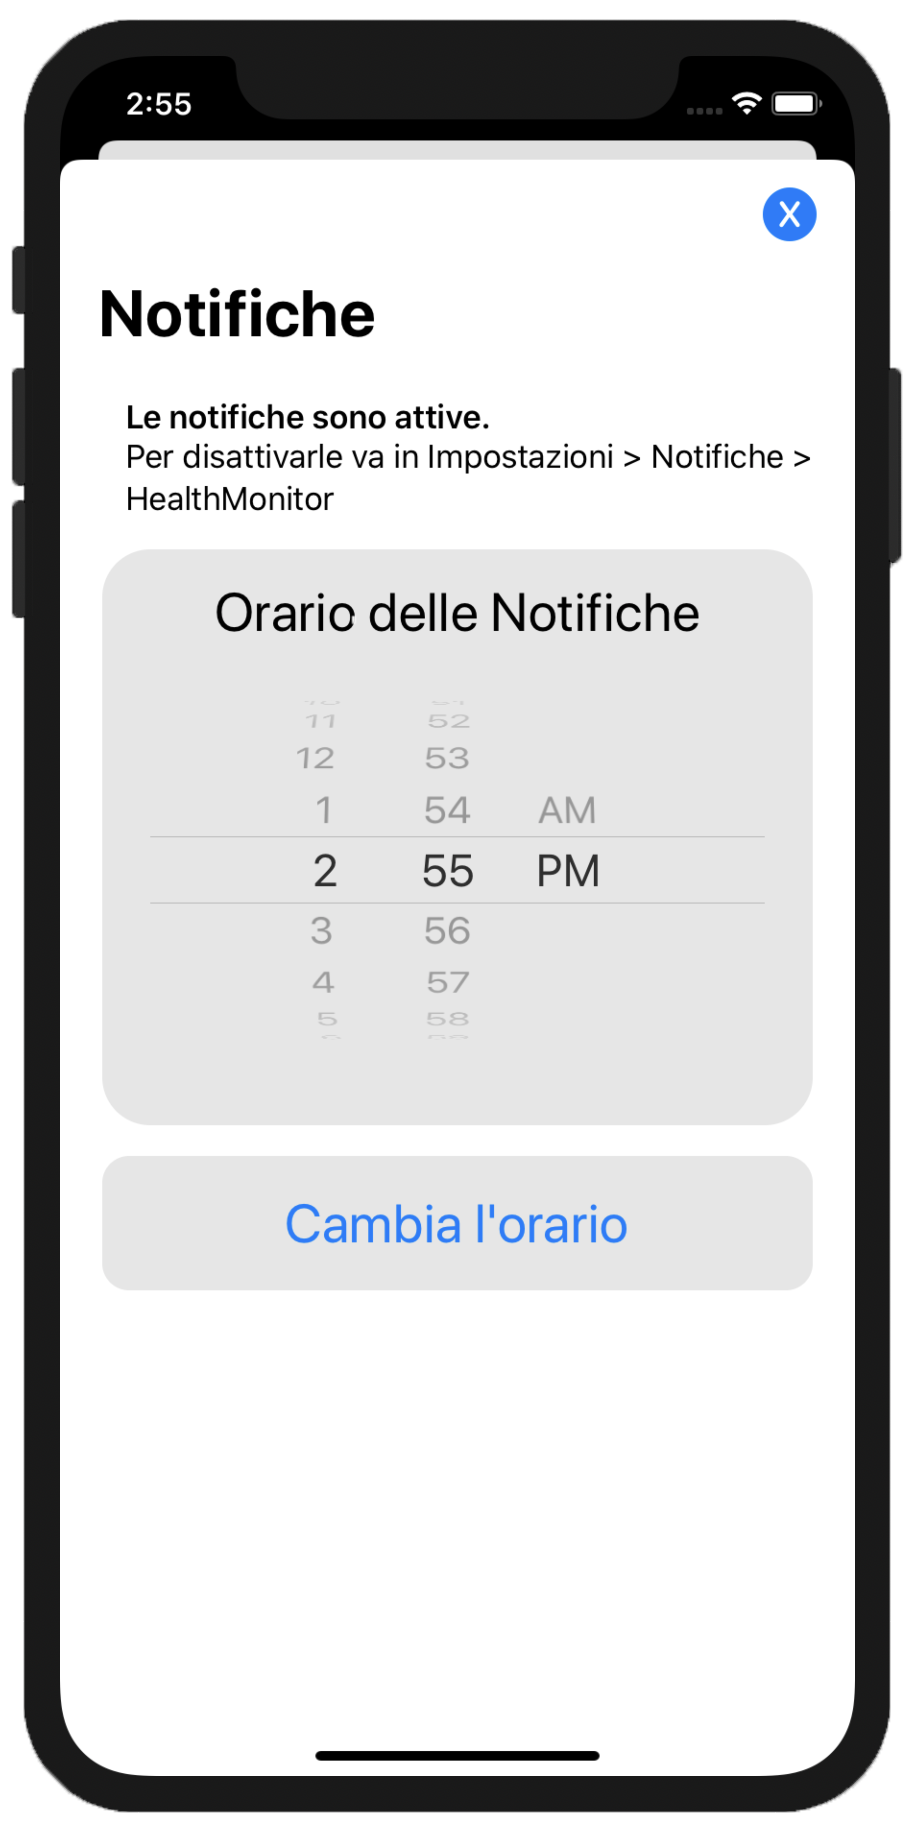
\includegraphics[width=.32\textwidth]{img/notifiche2.png}\hfill
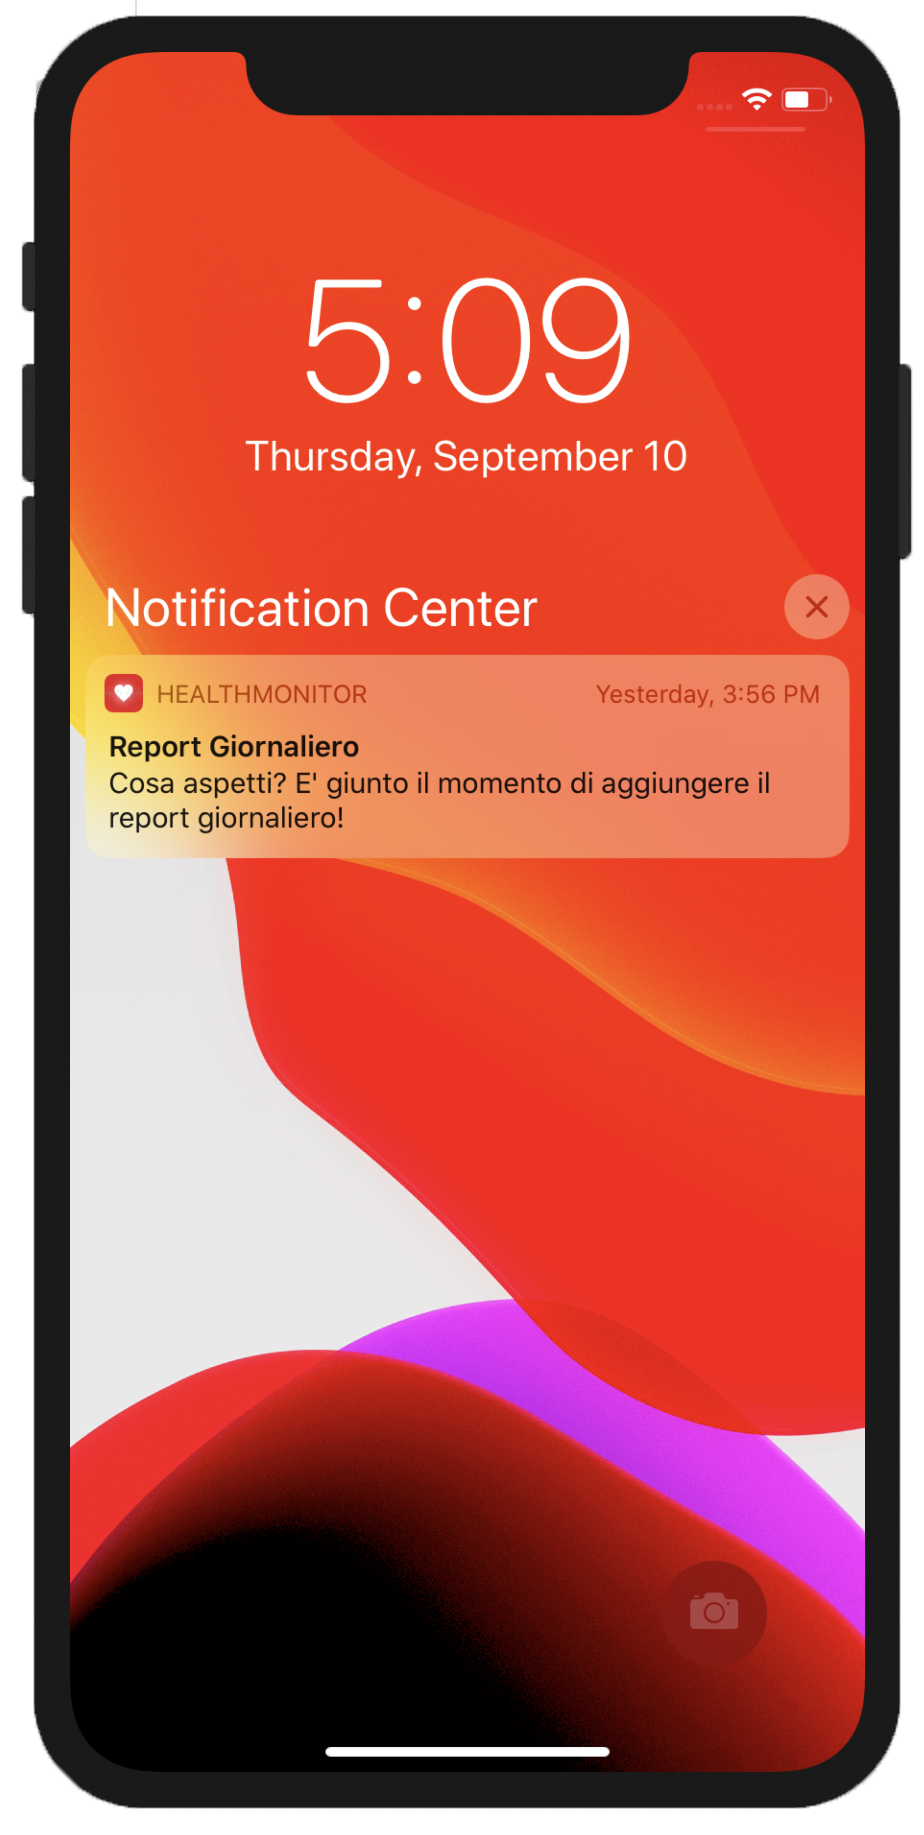
\includegraphics[width=.32\textwidth]{img/notifiche3.png}

\caption{Notifiche disablitate/Notifiche abilitate/Notifica}
\label{fig:figure5}

\end{figure}







%----------------------------------------------------------------------------------------
%	BIBLIOGRAPHY
%----------------------------------------------------------------------------------------

\bibliographystyle{apalike}

\bibliography{sample}

%----------------------------------------------------------------------------------------


\end{document}